% Created by tikzDevice version 0.9 on 2016-01-12 22:38:43
% !TEX encoding = UTF-8 Unicode
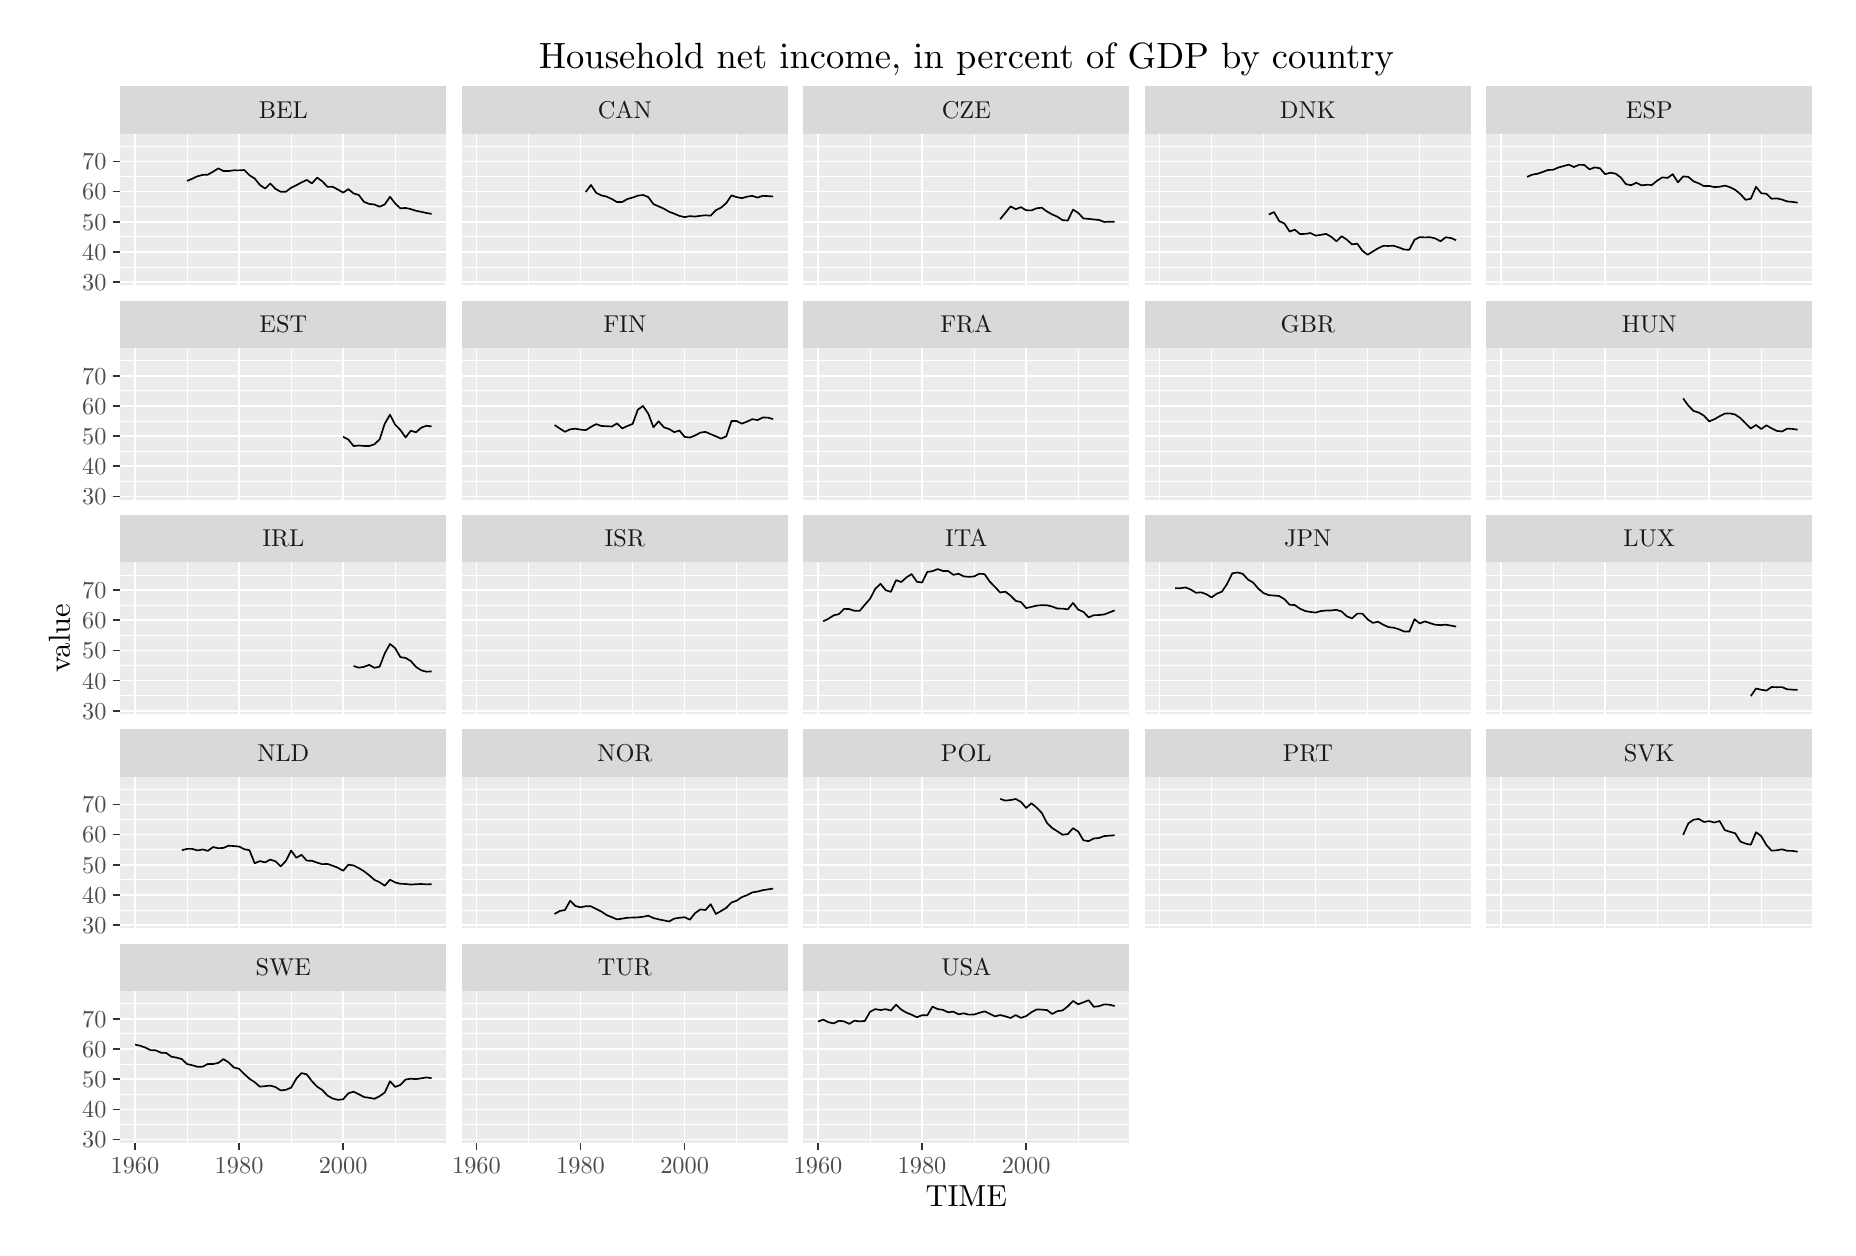
\begin{tikzpicture}[x=1pt,y=1pt]
\definecolor{fillColor}{RGB}{255,255,255}
\path[use as bounding box,fill=fillColor,fill opacity=0.00] (0,0) rectangle (650.43,433.62);
\begin{scope}
\path[clip] (  0.00,  0.00) rectangle (650.43,433.62);
\definecolor{drawColor}{RGB}{255,255,255}
\definecolor{fillColor}{RGB}{255,255,255}

\path[draw=drawColor,line width= 0.6pt,line join=round,line cap=round,fill=fillColor] (  0.00,  0.00) rectangle (650.43,433.62);
\end{scope}
\begin{scope}
\path[clip] ( 33.42,340.48) rectangle (151.33,395.37);
\definecolor{fillColor}{gray}{0.92}

\path[fill=fillColor] ( 33.42,340.48) rectangle (151.33,395.37);
\definecolor{drawColor}{RGB}{255,255,255}

\path[draw=drawColor,line width= 0.3pt,line join=round] ( 33.42,347.10) --
	(151.33,347.10);

\path[draw=drawColor,line width= 0.3pt,line join=round] ( 33.42,358.01) --
	(151.33,358.01);

\path[draw=drawColor,line width= 0.3pt,line join=round] ( 33.42,368.92) --
	(151.33,368.92);

\path[draw=drawColor,line width= 0.3pt,line join=round] ( 33.42,379.84) --
	(151.33,379.84);

\path[draw=drawColor,line width= 0.3pt,line join=round] ( 33.42,390.75) --
	(151.33,390.75);

\path[draw=drawColor,line width= 0.3pt,line join=round] ( 57.59,340.48) --
	( 57.59,395.37);

\path[draw=drawColor,line width= 0.3pt,line join=round] ( 95.20,340.48) --
	( 95.20,395.37);

\path[draw=drawColor,line width= 0.3pt,line join=round] (132.80,340.48) --
	(132.80,395.37);

\path[draw=drawColor,line width= 0.6pt,line join=round] ( 33.42,341.64) --
	(151.33,341.64);

\path[draw=drawColor,line width= 0.6pt,line join=round] ( 33.42,352.55) --
	(151.33,352.55);

\path[draw=drawColor,line width= 0.6pt,line join=round] ( 33.42,363.47) --
	(151.33,363.47);

\path[draw=drawColor,line width= 0.6pt,line join=round] ( 33.42,374.38) --
	(151.33,374.38);

\path[draw=drawColor,line width= 0.6pt,line join=round] ( 33.42,385.30) --
	(151.33,385.30);

\path[draw=drawColor,line width= 0.6pt,line join=round] ( 38.78,340.48) --
	( 38.78,395.37);

\path[draw=drawColor,line width= 0.6pt,line join=round] ( 76.39,340.48) --
	( 76.39,395.37);

\path[draw=drawColor,line width= 0.6pt,line join=round] (114.00,340.48) --
	(114.00,395.37);
\definecolor{drawColor}{RGB}{0,0,0}

\path[draw=drawColor,line width= 0.6pt,line join=round] ( 57.59,378.24) --
	( 59.47,379.03) --
	( 61.35,379.94) --
	( 63.23,380.40) --
	( 65.11,380.50) --
	( 66.99,381.57) --
	( 68.87,382.76) --
	( 70.75,381.81) --
	( 72.63,381.80) --
	( 74.51,382.08) --
	( 76.39,382.05) --
	( 78.27,382.19) --
	( 80.15,380.27) --
	( 82.03,379.12) --
	( 83.91,376.79) --
	( 85.79,375.48) --
	( 87.67,377.29) --
	( 89.55,375.37) --
	( 91.43,374.31) --
	( 93.31,374.35) --
	( 95.20,375.75) --
	( 97.08,376.70) --
	( 98.96,377.70) --
	(100.84,378.59) --
	(102.72,377.35) --
	(104.60,379.43) --
	(106.48,378.08) --
	(108.36,376.09) --
	(110.24,376.11) --
	(112.12,375.10) --
	(114.00,374.02) --
	(115.88,375.27) --
	(117.76,373.72) --
	(119.64,373.16) --
	(121.52,370.68) --
	(123.40,369.92) --
	(125.28,369.73) --
	(127.16,368.92) --
	(129.04,369.76) --
	(130.92,372.51) --
	(132.80,370.08) --
	(134.68,368.33) --
	(136.56,368.48) --
	(138.44,368.06) --
	(140.32,367.45) --
	(142.21,367.07) --
	(144.09,366.64) --
	(145.97,366.34);
\end{scope}
\begin{scope}
\path[clip] (156.83,340.48) rectangle (274.73,395.37);
\definecolor{fillColor}{gray}{0.92}

\path[fill=fillColor] (156.83,340.48) rectangle (274.73,395.37);
\definecolor{drawColor}{RGB}{255,255,255}

\path[draw=drawColor,line width= 0.3pt,line join=round] (156.83,347.10) --
	(274.73,347.10);

\path[draw=drawColor,line width= 0.3pt,line join=round] (156.83,358.01) --
	(274.73,358.01);

\path[draw=drawColor,line width= 0.3pt,line join=round] (156.83,368.92) --
	(274.73,368.92);

\path[draw=drawColor,line width= 0.3pt,line join=round] (156.83,379.84) --
	(274.73,379.84);

\path[draw=drawColor,line width= 0.3pt,line join=round] (156.83,390.75) --
	(274.73,390.75);

\path[draw=drawColor,line width= 0.3pt,line join=round] (180.99,340.48) --
	(180.99,395.37);

\path[draw=drawColor,line width= 0.3pt,line join=round] (218.60,340.48) --
	(218.60,395.37);

\path[draw=drawColor,line width= 0.3pt,line join=round] (256.20,340.48) --
	(256.20,395.37);

\path[draw=drawColor,line width= 0.6pt,line join=round] (156.83,341.64) --
	(274.73,341.64);

\path[draw=drawColor,line width= 0.6pt,line join=round] (156.83,352.55) --
	(274.73,352.55);

\path[draw=drawColor,line width= 0.6pt,line join=round] (156.83,363.47) --
	(274.73,363.47);

\path[draw=drawColor,line width= 0.6pt,line join=round] (156.83,374.38) --
	(274.73,374.38);

\path[draw=drawColor,line width= 0.6pt,line join=round] (156.83,385.30) --
	(274.73,385.30);

\path[draw=drawColor,line width= 0.6pt,line join=round] (162.18,340.48) --
	(162.18,395.37);

\path[draw=drawColor,line width= 0.6pt,line join=round] (199.79,340.48) --
	(199.79,395.37);

\path[draw=drawColor,line width= 0.6pt,line join=round] (237.40,340.48) --
	(237.40,395.37);
\definecolor{drawColor}{RGB}{0,0,0}

\path[draw=drawColor,line width= 0.6pt,line join=round] (201.67,374.27) --
	(203.55,376.77) --
	(205.43,373.92) --
	(207.31,373.00) --
	(209.19,372.57) --
	(211.07,371.71) --
	(212.96,370.59) --
	(214.84,370.63) --
	(216.72,371.69) --
	(218.60,372.22) --
	(220.48,372.91) --
	(222.36,373.16) --
	(224.24,372.42) --
	(226.12,369.85) --
	(228.00,369.06) --
	(229.88,368.20) --
	(231.76,367.10) --
	(233.64,366.40) --
	(235.52,365.60) --
	(237.40,365.15) --
	(239.28,365.53) --
	(241.16,365.36) --
	(243.04,365.63) --
	(244.92,365.82) --
	(246.80,365.68) --
	(248.68,367.66) --
	(250.56,368.59) --
	(252.44,370.22) --
	(254.32,373.01) --
	(256.20,372.38) --
	(258.08,372.01) --
	(259.97,372.55) --
	(261.85,372.84) --
	(263.73,372.23) --
	(265.61,372.84) --
	(267.49,372.75) --
	(269.37,372.62);
\end{scope}
\begin{scope}
\path[clip] (280.23,340.48) rectangle (398.13,395.37);
\definecolor{fillColor}{gray}{0.92}

\path[fill=fillColor] (280.23,340.48) rectangle (398.13,395.37);
\definecolor{drawColor}{RGB}{255,255,255}

\path[draw=drawColor,line width= 0.3pt,line join=round] (280.23,347.10) --
	(398.13,347.10);

\path[draw=drawColor,line width= 0.3pt,line join=round] (280.23,358.01) --
	(398.13,358.01);

\path[draw=drawColor,line width= 0.3pt,line join=round] (280.23,368.92) --
	(398.13,368.92);

\path[draw=drawColor,line width= 0.3pt,line join=round] (280.23,379.84) --
	(398.13,379.84);

\path[draw=drawColor,line width= 0.3pt,line join=round] (280.23,390.75) --
	(398.13,390.75);

\path[draw=drawColor,line width= 0.3pt,line join=round] (304.39,340.48) --
	(304.39,395.37);

\path[draw=drawColor,line width= 0.3pt,line join=round] (342.00,340.48) --
	(342.00,395.37);

\path[draw=drawColor,line width= 0.3pt,line join=round] (379.61,340.48) --
	(379.61,395.37);

\path[draw=drawColor,line width= 0.6pt,line join=round] (280.23,341.64) --
	(398.13,341.64);

\path[draw=drawColor,line width= 0.6pt,line join=round] (280.23,352.55) --
	(398.13,352.55);

\path[draw=drawColor,line width= 0.6pt,line join=round] (280.23,363.47) --
	(398.13,363.47);

\path[draw=drawColor,line width= 0.6pt,line join=round] (280.23,374.38) --
	(398.13,374.38);

\path[draw=drawColor,line width= 0.6pt,line join=round] (280.23,385.30) --
	(398.13,385.30);

\path[draw=drawColor,line width= 0.6pt,line join=round] (285.59,340.48) --
	(285.59,395.37);

\path[draw=drawColor,line width= 0.6pt,line join=round] (323.19,340.48) --
	(323.19,395.37);

\path[draw=drawColor,line width= 0.6pt,line join=round] (360.80,340.48) --
	(360.80,395.37);
\definecolor{drawColor}{RGB}{0,0,0}

\path[draw=drawColor,line width= 0.6pt,line join=round] (351.40,364.41) --
	(353.28,366.70) --
	(355.16,369.04) --
	(357.04,368.02) --
	(358.92,368.75) --
	(360.80,367.63) --
	(362.68,367.58) --
	(364.56,368.34) --
	(366.44,368.57) --
	(368.32,367.19) --
	(370.20,366.12) --
	(372.08,365.32) --
	(373.96,364.05) --
	(375.84,363.93) --
	(377.73,367.86) --
	(379.61,366.69) --
	(381.49,364.68) --
	(383.37,364.52) --
	(385.25,364.31) --
	(387.13,364.15) --
	(389.01,363.40) --
	(390.89,363.51) --
	(392.77,363.50);
\end{scope}
\begin{scope}
\path[clip] (403.63,340.48) rectangle (521.53,395.37);
\definecolor{fillColor}{gray}{0.92}

\path[fill=fillColor] (403.63,340.48) rectangle (521.53,395.37);
\definecolor{drawColor}{RGB}{255,255,255}

\path[draw=drawColor,line width= 0.3pt,line join=round] (403.63,347.10) --
	(521.53,347.10);

\path[draw=drawColor,line width= 0.3pt,line join=round] (403.63,358.01) --
	(521.53,358.01);

\path[draw=drawColor,line width= 0.3pt,line join=round] (403.63,368.92) --
	(521.53,368.92);

\path[draw=drawColor,line width= 0.3pt,line join=round] (403.63,379.84) --
	(521.53,379.84);

\path[draw=drawColor,line width= 0.3pt,line join=round] (403.63,390.75) --
	(521.53,390.75);

\path[draw=drawColor,line width= 0.3pt,line join=round] (427.79,340.48) --
	(427.79,395.37);

\path[draw=drawColor,line width= 0.3pt,line join=round] (465.40,340.48) --
	(465.40,395.37);

\path[draw=drawColor,line width= 0.3pt,line join=round] (503.01,340.48) --
	(503.01,395.37);

\path[draw=drawColor,line width= 0.6pt,line join=round] (403.63,341.64) --
	(521.53,341.64);

\path[draw=drawColor,line width= 0.6pt,line join=round] (403.63,352.55) --
	(521.53,352.55);

\path[draw=drawColor,line width= 0.6pt,line join=round] (403.63,363.47) --
	(521.53,363.47);

\path[draw=drawColor,line width= 0.6pt,line join=round] (403.63,374.38) --
	(521.53,374.38);

\path[draw=drawColor,line width= 0.6pt,line join=round] (403.63,385.30) --
	(521.53,385.30);

\path[draw=drawColor,line width= 0.6pt,line join=round] (408.99,340.48) --
	(408.99,395.37);

\path[draw=drawColor,line width= 0.6pt,line join=round] (446.59,340.48) --
	(446.59,395.37);

\path[draw=drawColor,line width= 0.6pt,line join=round] (484.20,340.48) --
	(484.20,395.37);
\definecolor{drawColor}{RGB}{0,0,0}

\path[draw=drawColor,line width= 0.6pt,line join=round] (448.48,366.10) --
	(450.36,366.98) --
	(452.24,363.72) --
	(454.12,362.84) --
	(456.00,359.95) --
	(457.88,360.61) --
	(459.76,359.04) --
	(461.64,359.10) --
	(463.52,359.41) --
	(465.40,358.47) --
	(467.28,358.75) --
	(469.16,359.12) --
	(471.04,358.03) --
	(472.92,356.42) --
	(474.80,358.24) --
	(476.68,357.00) --
	(478.56,355.31) --
	(480.44,355.56) --
	(482.32,352.99) --
	(484.20,351.56) --
	(486.08,352.74) --
	(487.96,353.90) --
	(489.84,354.78) --
	(491.72,354.74) --
	(493.60,354.83) --
	(495.49,354.20) --
	(497.37,353.45) --
	(499.25,353.35) --
	(501.13,356.99) --
	(503.01,357.93) --
	(504.89,357.83) --
	(506.77,357.89) --
	(508.65,357.45) --
	(510.53,356.43) --
	(512.41,357.88) --
	(514.29,357.59) --
	(516.17,356.82);
\end{scope}
\begin{scope}
\path[clip] (527.03,340.48) rectangle (644.93,395.37);
\definecolor{fillColor}{gray}{0.92}

\path[fill=fillColor] (527.03,340.48) rectangle (644.93,395.37);
\definecolor{drawColor}{RGB}{255,255,255}

\path[draw=drawColor,line width= 0.3pt,line join=round] (527.03,347.10) --
	(644.93,347.10);

\path[draw=drawColor,line width= 0.3pt,line join=round] (527.03,358.01) --
	(644.93,358.01);

\path[draw=drawColor,line width= 0.3pt,line join=round] (527.03,368.92) --
	(644.93,368.92);

\path[draw=drawColor,line width= 0.3pt,line join=round] (527.03,379.84) --
	(644.93,379.84);

\path[draw=drawColor,line width= 0.3pt,line join=round] (527.03,390.75) --
	(644.93,390.75);

\path[draw=drawColor,line width= 0.3pt,line join=round] (551.19,340.48) --
	(551.19,395.37);

\path[draw=drawColor,line width= 0.3pt,line join=round] (588.80,340.48) --
	(588.80,395.37);

\path[draw=drawColor,line width= 0.3pt,line join=round] (626.41,340.48) --
	(626.41,395.37);

\path[draw=drawColor,line width= 0.6pt,line join=round] (527.03,341.64) --
	(644.93,341.64);

\path[draw=drawColor,line width= 0.6pt,line join=round] (527.03,352.55) --
	(644.93,352.55);

\path[draw=drawColor,line width= 0.6pt,line join=round] (527.03,363.47) --
	(644.93,363.47);

\path[draw=drawColor,line width= 0.6pt,line join=round] (527.03,374.38) --
	(644.93,374.38);

\path[draw=drawColor,line width= 0.6pt,line join=round] (527.03,385.30) --
	(644.93,385.30);

\path[draw=drawColor,line width= 0.6pt,line join=round] (532.39,340.48) --
	(532.39,395.37);

\path[draw=drawColor,line width= 0.6pt,line join=round] (570.00,340.48) --
	(570.00,395.37);

\path[draw=drawColor,line width= 0.6pt,line join=round] (607.60,340.48) --
	(607.60,395.37);
\definecolor{drawColor}{RGB}{0,0,0}

\path[draw=drawColor,line width= 0.6pt,line join=round] (541.79,379.71) --
	(543.67,380.50) --
	(545.55,380.83) --
	(547.43,381.45) --
	(549.31,382.19) --
	(551.19,382.25) --
	(553.07,383.08) --
	(554.95,383.59) --
	(556.83,384.14) --
	(558.71,383.26) --
	(560.59,384.06) --
	(562.47,384.01) --
	(564.35,382.41) --
	(566.24,383.14) --
	(568.12,382.81) --
	(570.00,380.69) --
	(571.88,381.19) --
	(573.76,380.88) --
	(575.64,379.52) --
	(577.52,377.07) --
	(579.40,376.69) --
	(581.28,377.59) --
	(583.16,376.64) --
	(585.04,376.84) --
	(586.92,376.77) --
	(588.80,378.32) --
	(590.68,379.53) --
	(592.56,379.32) --
	(594.44,380.67) --
	(596.32,377.72) --
	(598.20,379.87) --
	(600.08,379.68) --
	(601.96,378.10) --
	(603.84,377.34) --
	(605.72,376.38) --
	(607.60,376.43) --
	(609.48,376.01) --
	(611.36,376.12) --
	(613.25,376.56) --
	(615.13,375.95) --
	(617.01,375.01) --
	(618.89,373.47) --
	(620.77,371.40) --
	(622.65,371.81) --
	(624.53,376.12) --
	(626.41,373.79) --
	(628.29,373.59) --
	(630.17,371.80) --
	(632.05,371.93) --
	(633.93,371.50) --
	(635.81,370.82) --
	(637.69,370.66) --
	(639.57,370.37);
\end{scope}
\begin{scope}
\path[clip] ( 33.42,263.03) rectangle (151.33,317.92);
\definecolor{fillColor}{gray}{0.92}

\path[fill=fillColor] ( 33.42,263.03) rectangle (151.33,317.92);
\definecolor{drawColor}{RGB}{255,255,255}

\path[draw=drawColor,line width= 0.3pt,line join=round] ( 33.42,269.65) --
	(151.33,269.65);

\path[draw=drawColor,line width= 0.3pt,line join=round] ( 33.42,280.56) --
	(151.33,280.56);

\path[draw=drawColor,line width= 0.3pt,line join=round] ( 33.42,291.48) --
	(151.33,291.48);

\path[draw=drawColor,line width= 0.3pt,line join=round] ( 33.42,302.39) --
	(151.33,302.39);

\path[draw=drawColor,line width= 0.3pt,line join=round] ( 33.42,313.30) --
	(151.33,313.30);

\path[draw=drawColor,line width= 0.3pt,line join=round] ( 57.59,263.03) --
	( 57.59,317.92);

\path[draw=drawColor,line width= 0.3pt,line join=round] ( 95.20,263.03) --
	( 95.20,317.92);

\path[draw=drawColor,line width= 0.3pt,line join=round] (132.80,263.03) --
	(132.80,317.92);

\path[draw=drawColor,line width= 0.6pt,line join=round] ( 33.42,264.19) --
	(151.33,264.19);

\path[draw=drawColor,line width= 0.6pt,line join=round] ( 33.42,275.11) --
	(151.33,275.11);

\path[draw=drawColor,line width= 0.6pt,line join=round] ( 33.42,286.02) --
	(151.33,286.02);

\path[draw=drawColor,line width= 0.6pt,line join=round] ( 33.42,296.93) --
	(151.33,296.93);

\path[draw=drawColor,line width= 0.6pt,line join=round] ( 33.42,307.85) --
	(151.33,307.85);

\path[draw=drawColor,line width= 0.6pt,line join=round] ( 38.78,263.03) --
	( 38.78,317.92);

\path[draw=drawColor,line width= 0.6pt,line join=round] ( 76.39,263.03) --
	( 76.39,317.92);

\path[draw=drawColor,line width= 0.6pt,line join=round] (114.00,263.03) --
	(114.00,317.92);
\definecolor{drawColor}{RGB}{0,0,0}

\path[draw=drawColor,line width= 0.6pt,line join=round] (114.00,285.78) --
	(115.88,284.78) --
	(117.76,282.44) --
	(119.64,282.63) --
	(121.52,282.48) --
	(123.40,282.45) --
	(125.28,283.07) --
	(127.16,284.82) --
	(129.04,290.51) --
	(130.92,293.76) --
	(132.80,290.14) --
	(134.68,288.24) --
	(136.56,285.55) --
	(138.44,287.98) --
	(140.32,287.41) --
	(142.21,289.07) --
	(144.09,289.76) --
	(145.97,289.54);
\end{scope}
\begin{scope}
\path[clip] (156.83,263.03) rectangle (274.73,317.92);
\definecolor{fillColor}{gray}{0.92}

\path[fill=fillColor] (156.83,263.03) rectangle (274.73,317.92);
\definecolor{drawColor}{RGB}{255,255,255}

\path[draw=drawColor,line width= 0.3pt,line join=round] (156.83,269.65) --
	(274.73,269.65);

\path[draw=drawColor,line width= 0.3pt,line join=round] (156.83,280.56) --
	(274.73,280.56);

\path[draw=drawColor,line width= 0.3pt,line join=round] (156.83,291.48) --
	(274.73,291.48);

\path[draw=drawColor,line width= 0.3pt,line join=round] (156.83,302.39) --
	(274.73,302.39);

\path[draw=drawColor,line width= 0.3pt,line join=round] (156.83,313.30) --
	(274.73,313.30);

\path[draw=drawColor,line width= 0.3pt,line join=round] (180.99,263.03) --
	(180.99,317.92);

\path[draw=drawColor,line width= 0.3pt,line join=round] (218.60,263.03) --
	(218.60,317.92);

\path[draw=drawColor,line width= 0.3pt,line join=round] (256.20,263.03) --
	(256.20,317.92);

\path[draw=drawColor,line width= 0.6pt,line join=round] (156.83,264.19) --
	(274.73,264.19);

\path[draw=drawColor,line width= 0.6pt,line join=round] (156.83,275.11) --
	(274.73,275.11);

\path[draw=drawColor,line width= 0.6pt,line join=round] (156.83,286.02) --
	(274.73,286.02);

\path[draw=drawColor,line width= 0.6pt,line join=round] (156.83,296.93) --
	(274.73,296.93);

\path[draw=drawColor,line width= 0.6pt,line join=round] (156.83,307.85) --
	(274.73,307.85);

\path[draw=drawColor,line width= 0.6pt,line join=round] (162.18,263.03) --
	(162.18,317.92);

\path[draw=drawColor,line width= 0.6pt,line join=round] (199.79,263.03) --
	(199.79,317.92);

\path[draw=drawColor,line width= 0.6pt,line join=round] (237.40,263.03) --
	(237.40,317.92);
\definecolor{drawColor}{RGB}{0,0,0}

\path[draw=drawColor,line width= 0.6pt,line join=round] (190.39,290.03) --
	(192.27,288.78) --
	(194.15,287.59) --
	(196.03,288.49) --
	(197.91,288.69) --
	(199.79,288.37) --
	(201.67,288.17) --
	(203.55,289.37) --
	(205.43,290.37) --
	(207.31,289.68) --
	(209.19,289.61) --
	(211.07,289.49) --
	(212.96,290.61) --
	(214.84,288.82) --
	(216.72,289.68) --
	(218.60,290.43) --
	(220.48,295.59) --
	(222.36,296.91) --
	(224.24,294.15) --
	(226.12,289.23) --
	(228.00,291.38) --
	(229.88,289.23) --
	(231.76,288.60) --
	(233.64,287.45) --
	(235.52,288.04) --
	(237.40,285.75) --
	(239.28,285.51) --
	(241.16,286.24) --
	(243.04,287.28) --
	(244.92,287.57) --
	(246.80,286.73) --
	(248.68,285.97) --
	(250.56,285.12) --
	(252.44,285.94) --
	(254.32,291.49) --
	(256.20,291.46) --
	(258.08,290.53) --
	(259.97,291.28) --
	(261.85,292.16) --
	(263.73,291.80) --
	(265.61,292.74) --
	(267.49,292.71) --
	(269.37,292.17);
\end{scope}
\begin{scope}
\path[clip] (280.23,263.03) rectangle (398.13,317.92);
\definecolor{fillColor}{gray}{0.92}

\path[fill=fillColor] (280.23,263.03) rectangle (398.13,317.92);
\definecolor{drawColor}{RGB}{255,255,255}

\path[draw=drawColor,line width= 0.3pt,line join=round] (280.23,269.65) --
	(398.13,269.65);

\path[draw=drawColor,line width= 0.3pt,line join=round] (280.23,280.56) --
	(398.13,280.56);

\path[draw=drawColor,line width= 0.3pt,line join=round] (280.23,291.48) --
	(398.13,291.48);

\path[draw=drawColor,line width= 0.3pt,line join=round] (280.23,302.39) --
	(398.13,302.39);

\path[draw=drawColor,line width= 0.3pt,line join=round] (280.23,313.30) --
	(398.13,313.30);

\path[draw=drawColor,line width= 0.3pt,line join=round] (304.39,263.03) --
	(304.39,317.92);

\path[draw=drawColor,line width= 0.3pt,line join=round] (342.00,263.03) --
	(342.00,317.92);

\path[draw=drawColor,line width= 0.3pt,line join=round] (379.61,263.03) --
	(379.61,317.92);

\path[draw=drawColor,line width= 0.6pt,line join=round] (280.23,264.19) --
	(398.13,264.19);

\path[draw=drawColor,line width= 0.6pt,line join=round] (280.23,275.11) --
	(398.13,275.11);

\path[draw=drawColor,line width= 0.6pt,line join=round] (280.23,286.02) --
	(398.13,286.02);

\path[draw=drawColor,line width= 0.6pt,line join=round] (280.23,296.93) --
	(398.13,296.93);

\path[draw=drawColor,line width= 0.6pt,line join=round] (280.23,307.85) --
	(398.13,307.85);

\path[draw=drawColor,line width= 0.6pt,line join=round] (285.59,263.03) --
	(285.59,317.92);

\path[draw=drawColor,line width= 0.6pt,line join=round] (323.19,263.03) --
	(323.19,317.92);

\path[draw=drawColor,line width= 0.6pt,line join=round] (360.80,263.03) --
	(360.80,317.92);
\end{scope}
\begin{scope}
\path[clip] (403.63,263.03) rectangle (521.53,317.92);
\definecolor{fillColor}{gray}{0.92}

\path[fill=fillColor] (403.63,263.03) rectangle (521.53,317.92);
\definecolor{drawColor}{RGB}{255,255,255}

\path[draw=drawColor,line width= 0.3pt,line join=round] (403.63,269.65) --
	(521.53,269.65);

\path[draw=drawColor,line width= 0.3pt,line join=round] (403.63,280.56) --
	(521.53,280.56);

\path[draw=drawColor,line width= 0.3pt,line join=round] (403.63,291.48) --
	(521.53,291.48);

\path[draw=drawColor,line width= 0.3pt,line join=round] (403.63,302.39) --
	(521.53,302.39);

\path[draw=drawColor,line width= 0.3pt,line join=round] (403.63,313.30) --
	(521.53,313.30);

\path[draw=drawColor,line width= 0.3pt,line join=round] (427.79,263.03) --
	(427.79,317.92);

\path[draw=drawColor,line width= 0.3pt,line join=round] (465.40,263.03) --
	(465.40,317.92);

\path[draw=drawColor,line width= 0.3pt,line join=round] (503.01,263.03) --
	(503.01,317.92);

\path[draw=drawColor,line width= 0.6pt,line join=round] (403.63,264.19) --
	(521.53,264.19);

\path[draw=drawColor,line width= 0.6pt,line join=round] (403.63,275.11) --
	(521.53,275.11);

\path[draw=drawColor,line width= 0.6pt,line join=round] (403.63,286.02) --
	(521.53,286.02);

\path[draw=drawColor,line width= 0.6pt,line join=round] (403.63,296.93) --
	(521.53,296.93);

\path[draw=drawColor,line width= 0.6pt,line join=round] (403.63,307.85) --
	(521.53,307.85);

\path[draw=drawColor,line width= 0.6pt,line join=round] (408.99,263.03) --
	(408.99,317.92);

\path[draw=drawColor,line width= 0.6pt,line join=round] (446.59,263.03) --
	(446.59,317.92);

\path[draw=drawColor,line width= 0.6pt,line join=round] (484.20,263.03) --
	(484.20,317.92);
\end{scope}
\begin{scope}
\path[clip] (527.03,263.03) rectangle (644.93,317.92);
\definecolor{fillColor}{gray}{0.92}

\path[fill=fillColor] (527.03,263.03) rectangle (644.93,317.92);
\definecolor{drawColor}{RGB}{255,255,255}

\path[draw=drawColor,line width= 0.3pt,line join=round] (527.03,269.65) --
	(644.93,269.65);

\path[draw=drawColor,line width= 0.3pt,line join=round] (527.03,280.56) --
	(644.93,280.56);

\path[draw=drawColor,line width= 0.3pt,line join=round] (527.03,291.48) --
	(644.93,291.48);

\path[draw=drawColor,line width= 0.3pt,line join=round] (527.03,302.39) --
	(644.93,302.39);

\path[draw=drawColor,line width= 0.3pt,line join=round] (527.03,313.30) --
	(644.93,313.30);

\path[draw=drawColor,line width= 0.3pt,line join=round] (551.19,263.03) --
	(551.19,317.92);

\path[draw=drawColor,line width= 0.3pt,line join=round] (588.80,263.03) --
	(588.80,317.92);

\path[draw=drawColor,line width= 0.3pt,line join=round] (626.41,263.03) --
	(626.41,317.92);

\path[draw=drawColor,line width= 0.6pt,line join=round] (527.03,264.19) --
	(644.93,264.19);

\path[draw=drawColor,line width= 0.6pt,line join=round] (527.03,275.11) --
	(644.93,275.11);

\path[draw=drawColor,line width= 0.6pt,line join=round] (527.03,286.02) --
	(644.93,286.02);

\path[draw=drawColor,line width= 0.6pt,line join=round] (527.03,296.93) --
	(644.93,296.93);

\path[draw=drawColor,line width= 0.6pt,line join=round] (527.03,307.85) --
	(644.93,307.85);

\path[draw=drawColor,line width= 0.6pt,line join=round] (532.39,263.03) --
	(532.39,317.92);

\path[draw=drawColor,line width= 0.6pt,line join=round] (570.00,263.03) --
	(570.00,317.92);

\path[draw=drawColor,line width= 0.6pt,line join=round] (607.60,263.03) --
	(607.60,317.92);
\definecolor{drawColor}{RGB}{0,0,0}

\path[draw=drawColor,line width= 0.6pt,line join=round] (598.20,299.64) --
	(600.08,297.03) --
	(601.96,295.13) --
	(603.84,294.54) --
	(605.72,293.40) --
	(607.60,291.36) --
	(609.48,292.12) --
	(611.36,293.21) --
	(613.25,294.17) --
	(615.13,294.22) --
	(617.01,293.82) --
	(618.89,292.54) --
	(620.77,290.63) --
	(622.65,288.80) --
	(624.53,290.06) --
	(626.41,288.58) --
	(628.29,289.93) --
	(630.17,288.84) --
	(632.05,287.92) --
	(633.93,287.70) --
	(635.81,288.74) --
	(637.69,288.62) --
	(639.57,288.35);
\end{scope}
\begin{scope}
\path[clip] ( 33.42,185.58) rectangle (151.33,240.47);
\definecolor{fillColor}{gray}{0.92}

\path[fill=fillColor] ( 33.42,185.58) rectangle (151.33,240.47);
\definecolor{drawColor}{RGB}{255,255,255}

\path[draw=drawColor,line width= 0.3pt,line join=round] ( 33.42,192.20) --
	(151.33,192.20);

\path[draw=drawColor,line width= 0.3pt,line join=round] ( 33.42,203.11) --
	(151.33,203.11);

\path[draw=drawColor,line width= 0.3pt,line join=round] ( 33.42,214.03) --
	(151.33,214.03);

\path[draw=drawColor,line width= 0.3pt,line join=round] ( 33.42,224.94) --
	(151.33,224.94);

\path[draw=drawColor,line width= 0.3pt,line join=round] ( 33.42,235.86) --
	(151.33,235.86);

\path[draw=drawColor,line width= 0.3pt,line join=round] ( 57.59,185.58) --
	( 57.59,240.47);

\path[draw=drawColor,line width= 0.3pt,line join=round] ( 95.20,185.58) --
	( 95.20,240.47);

\path[draw=drawColor,line width= 0.3pt,line join=round] (132.80,185.58) --
	(132.80,240.47);

\path[draw=drawColor,line width= 0.6pt,line join=round] ( 33.42,186.74) --
	(151.33,186.74);

\path[draw=drawColor,line width= 0.6pt,line join=round] ( 33.42,197.66) --
	(151.33,197.66);

\path[draw=drawColor,line width= 0.6pt,line join=round] ( 33.42,208.57) --
	(151.33,208.57);

\path[draw=drawColor,line width= 0.6pt,line join=round] ( 33.42,219.49) --
	(151.33,219.49);

\path[draw=drawColor,line width= 0.6pt,line join=round] ( 33.42,230.40) --
	(151.33,230.40);

\path[draw=drawColor,line width= 0.6pt,line join=round] ( 38.78,185.58) --
	( 38.78,240.47);

\path[draw=drawColor,line width= 0.6pt,line join=round] ( 76.39,185.58) --
	( 76.39,240.47);

\path[draw=drawColor,line width= 0.6pt,line join=round] (114.00,185.58) --
	(114.00,240.47);
\definecolor{drawColor}{RGB}{0,0,0}

\path[draw=drawColor,line width= 0.6pt,line join=round] (117.76,202.96) --
	(119.64,202.35) --
	(121.52,202.64) --
	(123.40,203.37) --
	(125.28,202.31) --
	(127.16,202.70) --
	(129.04,207.52) --
	(130.92,210.92) --
	(132.80,209.40) --
	(134.68,206.15) --
	(136.56,205.88) --
	(138.44,204.75) --
	(140.32,202.63) --
	(142.21,201.40) --
	(144.09,200.90) --
	(145.97,200.98);
\end{scope}
\begin{scope}
\path[clip] (156.83,185.58) rectangle (274.73,240.47);
\definecolor{fillColor}{gray}{0.92}

\path[fill=fillColor] (156.83,185.58) rectangle (274.73,240.47);
\definecolor{drawColor}{RGB}{255,255,255}

\path[draw=drawColor,line width= 0.3pt,line join=round] (156.83,192.20) --
	(274.73,192.20);

\path[draw=drawColor,line width= 0.3pt,line join=round] (156.83,203.11) --
	(274.73,203.11);

\path[draw=drawColor,line width= 0.3pt,line join=round] (156.83,214.03) --
	(274.73,214.03);

\path[draw=drawColor,line width= 0.3pt,line join=round] (156.83,224.94) --
	(274.73,224.94);

\path[draw=drawColor,line width= 0.3pt,line join=round] (156.83,235.86) --
	(274.73,235.86);

\path[draw=drawColor,line width= 0.3pt,line join=round] (180.99,185.58) --
	(180.99,240.47);

\path[draw=drawColor,line width= 0.3pt,line join=round] (218.60,185.58) --
	(218.60,240.47);

\path[draw=drawColor,line width= 0.3pt,line join=round] (256.20,185.58) --
	(256.20,240.47);

\path[draw=drawColor,line width= 0.6pt,line join=round] (156.83,186.74) --
	(274.73,186.74);

\path[draw=drawColor,line width= 0.6pt,line join=round] (156.83,197.66) --
	(274.73,197.66);

\path[draw=drawColor,line width= 0.6pt,line join=round] (156.83,208.57) --
	(274.73,208.57);

\path[draw=drawColor,line width= 0.6pt,line join=round] (156.83,219.49) --
	(274.73,219.49);

\path[draw=drawColor,line width= 0.6pt,line join=round] (156.83,230.40) --
	(274.73,230.40);

\path[draw=drawColor,line width= 0.6pt,line join=round] (162.18,185.58) --
	(162.18,240.47);

\path[draw=drawColor,line width= 0.6pt,line join=round] (199.79,185.58) --
	(199.79,240.47);

\path[draw=drawColor,line width= 0.6pt,line join=round] (237.40,185.58) --
	(237.40,240.47);
\end{scope}
\begin{scope}
\path[clip] (280.23,185.58) rectangle (398.13,240.47);
\definecolor{fillColor}{gray}{0.92}

\path[fill=fillColor] (280.23,185.58) rectangle (398.13,240.47);
\definecolor{drawColor}{RGB}{255,255,255}

\path[draw=drawColor,line width= 0.3pt,line join=round] (280.23,192.20) --
	(398.13,192.20);

\path[draw=drawColor,line width= 0.3pt,line join=round] (280.23,203.11) --
	(398.13,203.11);

\path[draw=drawColor,line width= 0.3pt,line join=round] (280.23,214.03) --
	(398.13,214.03);

\path[draw=drawColor,line width= 0.3pt,line join=round] (280.23,224.94) --
	(398.13,224.94);

\path[draw=drawColor,line width= 0.3pt,line join=round] (280.23,235.86) --
	(398.13,235.86);

\path[draw=drawColor,line width= 0.3pt,line join=round] (304.39,185.58) --
	(304.39,240.47);

\path[draw=drawColor,line width= 0.3pt,line join=round] (342.00,185.58) --
	(342.00,240.47);

\path[draw=drawColor,line width= 0.3pt,line join=round] (379.61,185.58) --
	(379.61,240.47);

\path[draw=drawColor,line width= 0.6pt,line join=round] (280.23,186.74) --
	(398.13,186.74);

\path[draw=drawColor,line width= 0.6pt,line join=round] (280.23,197.66) --
	(398.13,197.66);

\path[draw=drawColor,line width= 0.6pt,line join=round] (280.23,208.57) --
	(398.13,208.57);

\path[draw=drawColor,line width= 0.6pt,line join=round] (280.23,219.49) --
	(398.13,219.49);

\path[draw=drawColor,line width= 0.6pt,line join=round] (280.23,230.40) --
	(398.13,230.40);

\path[draw=drawColor,line width= 0.6pt,line join=round] (285.59,185.58) --
	(285.59,240.47);

\path[draw=drawColor,line width= 0.6pt,line join=round] (323.19,185.58) --
	(323.19,240.47);

\path[draw=drawColor,line width= 0.6pt,line join=round] (360.80,185.58) --
	(360.80,240.47);
\definecolor{drawColor}{RGB}{0,0,0}

\path[draw=drawColor,line width= 0.6pt,line join=round] (287.47,219.12) --
	(289.35,220.03) --
	(291.23,221.26) --
	(293.11,221.69) --
	(294.99,223.60) --
	(296.87,223.53) --
	(298.75,222.91) --
	(300.63,222.88) --
	(302.51,225.09) --
	(304.39,227.26) --
	(306.27,230.82) --
	(308.15,232.67) --
	(310.03,230.36) --
	(311.91,229.75) --
	(313.79,233.98) --
	(315.67,233.30) --
	(317.55,234.98) --
	(319.43,236.18) --
	(321.31,233.39) --
	(323.19,233.13) --
	(325.07,236.94) --
	(326.95,237.23) --
	(328.83,237.98) --
	(330.72,237.29) --
	(332.60,237.29) --
	(334.48,235.88) --
	(336.36,236.30) --
	(338.24,235.35) --
	(340.12,235.17) --
	(342.00,235.33) --
	(343.88,236.31) --
	(345.76,236.15) --
	(347.64,233.45) --
	(349.52,231.53) --
	(351.40,229.52) --
	(353.28,229.82) --
	(355.16,228.39) --
	(357.04,226.48) --
	(358.92,226.05) --
	(360.80,223.89) --
	(362.68,224.31) --
	(364.56,224.76) --
	(366.44,224.95) --
	(368.32,224.90) --
	(370.20,224.44) --
	(372.08,223.72) --
	(373.96,223.69) --
	(375.84,223.43) --
	(377.73,225.75) --
	(379.61,223.32) --
	(381.49,222.52) --
	(383.37,220.53) --
	(385.25,221.32) --
	(387.13,221.37) --
	(389.01,221.59) --
	(390.89,222.32) --
	(392.77,223.05);
\end{scope}
\begin{scope}
\path[clip] (403.63,185.58) rectangle (521.53,240.47);
\definecolor{fillColor}{gray}{0.92}

\path[fill=fillColor] (403.63,185.58) rectangle (521.53,240.47);
\definecolor{drawColor}{RGB}{255,255,255}

\path[draw=drawColor,line width= 0.3pt,line join=round] (403.63,192.20) --
	(521.53,192.20);

\path[draw=drawColor,line width= 0.3pt,line join=round] (403.63,203.11) --
	(521.53,203.11);

\path[draw=drawColor,line width= 0.3pt,line join=round] (403.63,214.03) --
	(521.53,214.03);

\path[draw=drawColor,line width= 0.3pt,line join=round] (403.63,224.94) --
	(521.53,224.94);

\path[draw=drawColor,line width= 0.3pt,line join=round] (403.63,235.86) --
	(521.53,235.86);

\path[draw=drawColor,line width= 0.3pt,line join=round] (427.79,185.58) --
	(427.79,240.47);

\path[draw=drawColor,line width= 0.3pt,line join=round] (465.40,185.58) --
	(465.40,240.47);

\path[draw=drawColor,line width= 0.3pt,line join=round] (503.01,185.58) --
	(503.01,240.47);

\path[draw=drawColor,line width= 0.6pt,line join=round] (403.63,186.74) --
	(521.53,186.74);

\path[draw=drawColor,line width= 0.6pt,line join=round] (403.63,197.66) --
	(521.53,197.66);

\path[draw=drawColor,line width= 0.6pt,line join=round] (403.63,208.57) --
	(521.53,208.57);

\path[draw=drawColor,line width= 0.6pt,line join=round] (403.63,219.49) --
	(521.53,219.49);

\path[draw=drawColor,line width= 0.6pt,line join=round] (403.63,230.40) --
	(521.53,230.40);

\path[draw=drawColor,line width= 0.6pt,line join=round] (408.99,185.58) --
	(408.99,240.47);

\path[draw=drawColor,line width= 0.6pt,line join=round] (446.59,185.58) --
	(446.59,240.47);

\path[draw=drawColor,line width= 0.6pt,line join=round] (484.20,185.58) --
	(484.20,240.47);
\definecolor{drawColor}{RGB}{0,0,0}

\path[draw=drawColor,line width= 0.6pt,line join=round] (414.63,231.07) --
	(416.51,231.06) --
	(418.39,231.34) --
	(420.27,230.59) --
	(422.15,229.42) --
	(424.03,229.58) --
	(425.91,228.90) --
	(427.79,227.73) --
	(429.67,229.08) --
	(431.55,229.82) --
	(433.43,232.67) --
	(435.31,236.43) --
	(437.19,236.77) --
	(439.07,236.25) --
	(440.95,234.19) --
	(442.83,233.10) --
	(444.71,230.88) --
	(446.59,229.30) --
	(448.48,228.57) --
	(450.36,228.42) --
	(452.24,228.24) --
	(454.12,227.12) --
	(456.00,225.09) --
	(457.88,224.97) --
	(459.76,223.66) --
	(461.64,222.82) --
	(463.52,222.49) --
	(465.40,222.27) --
	(467.28,222.82) --
	(469.16,223.00) --
	(471.04,223.03) --
	(472.92,223.27) --
	(474.80,222.65) --
	(476.68,220.89) --
	(478.56,220.17) --
	(480.44,221.89) --
	(482.32,221.86) --
	(484.20,219.81) --
	(486.08,218.54) --
	(487.96,218.96) --
	(489.84,217.87) --
	(491.72,217.02) --
	(493.60,216.81) --
	(495.49,216.22) --
	(497.37,215.43) --
	(499.25,215.39) --
	(501.13,219.88) --
	(503.01,218.33) --
	(504.89,219.09) --
	(506.77,218.43) --
	(508.65,217.86) --
	(510.53,217.73) --
	(512.41,217.89) --
	(514.29,217.56) --
	(516.17,217.20);
\end{scope}
\begin{scope}
\path[clip] (527.03,185.58) rectangle (644.93,240.47);
\definecolor{fillColor}{gray}{0.92}

\path[fill=fillColor] (527.03,185.58) rectangle (644.93,240.47);
\definecolor{drawColor}{RGB}{255,255,255}

\path[draw=drawColor,line width= 0.3pt,line join=round] (527.03,192.20) --
	(644.93,192.20);

\path[draw=drawColor,line width= 0.3pt,line join=round] (527.03,203.11) --
	(644.93,203.11);

\path[draw=drawColor,line width= 0.3pt,line join=round] (527.03,214.03) --
	(644.93,214.03);

\path[draw=drawColor,line width= 0.3pt,line join=round] (527.03,224.94) --
	(644.93,224.94);

\path[draw=drawColor,line width= 0.3pt,line join=round] (527.03,235.86) --
	(644.93,235.86);

\path[draw=drawColor,line width= 0.3pt,line join=round] (551.19,185.58) --
	(551.19,240.47);

\path[draw=drawColor,line width= 0.3pt,line join=round] (588.80,185.58) --
	(588.80,240.47);

\path[draw=drawColor,line width= 0.3pt,line join=round] (626.41,185.58) --
	(626.41,240.47);

\path[draw=drawColor,line width= 0.6pt,line join=round] (527.03,186.74) --
	(644.93,186.74);

\path[draw=drawColor,line width= 0.6pt,line join=round] (527.03,197.66) --
	(644.93,197.66);

\path[draw=drawColor,line width= 0.6pt,line join=round] (527.03,208.57) --
	(644.93,208.57);

\path[draw=drawColor,line width= 0.6pt,line join=round] (527.03,219.49) --
	(644.93,219.49);

\path[draw=drawColor,line width= 0.6pt,line join=round] (527.03,230.40) --
	(644.93,230.40);

\path[draw=drawColor,line width= 0.6pt,line join=round] (532.39,185.58) --
	(532.39,240.47);

\path[draw=drawColor,line width= 0.6pt,line join=round] (570.00,185.58) --
	(570.00,240.47);

\path[draw=drawColor,line width= 0.6pt,line join=round] (607.60,185.58) --
	(607.60,240.47);
\definecolor{drawColor}{RGB}{0,0,0}

\path[draw=drawColor,line width= 0.6pt,line join=round] (622.65,192.09) --
	(624.53,194.83) --
	(626.41,194.38) --
	(628.29,194.08) --
	(630.17,195.36) --
	(632.05,195.30) --
	(633.93,195.33) --
	(635.81,194.54) --
	(637.69,194.41) --
	(639.57,194.33);
\end{scope}
\begin{scope}
\path[clip] ( 33.42,108.14) rectangle (151.33,163.02);
\definecolor{fillColor}{gray}{0.92}

\path[fill=fillColor] ( 33.42,108.14) rectangle (151.33,163.02);
\definecolor{drawColor}{RGB}{255,255,255}

\path[draw=drawColor,line width= 0.3pt,line join=round] ( 33.42,114.75) --
	(151.33,114.75);

\path[draw=drawColor,line width= 0.3pt,line join=round] ( 33.42,125.67) --
	(151.33,125.67);

\path[draw=drawColor,line width= 0.3pt,line join=round] ( 33.42,136.58) --
	(151.33,136.58);

\path[draw=drawColor,line width= 0.3pt,line join=round] ( 33.42,147.49) --
	(151.33,147.49);

\path[draw=drawColor,line width= 0.3pt,line join=round] ( 33.42,158.41) --
	(151.33,158.41);

\path[draw=drawColor,line width= 0.3pt,line join=round] ( 57.59,108.14) --
	( 57.59,163.02);

\path[draw=drawColor,line width= 0.3pt,line join=round] ( 95.20,108.14) --
	( 95.20,163.02);

\path[draw=drawColor,line width= 0.3pt,line join=round] (132.80,108.14) --
	(132.80,163.02);

\path[draw=drawColor,line width= 0.6pt,line join=round] ( 33.42,109.29) --
	(151.33,109.29);

\path[draw=drawColor,line width= 0.6pt,line join=round] ( 33.42,120.21) --
	(151.33,120.21);

\path[draw=drawColor,line width= 0.6pt,line join=round] ( 33.42,131.12) --
	(151.33,131.12);

\path[draw=drawColor,line width= 0.6pt,line join=round] ( 33.42,142.04) --
	(151.33,142.04);

\path[draw=drawColor,line width= 0.6pt,line join=round] ( 33.42,152.95) --
	(151.33,152.95);

\path[draw=drawColor,line width= 0.6pt,line join=round] ( 38.78,108.14) --
	( 38.78,163.02);

\path[draw=drawColor,line width= 0.6pt,line join=round] ( 76.39,108.14) --
	( 76.39,163.02);

\path[draw=drawColor,line width= 0.6pt,line join=round] (114.00,108.14) --
	(114.00,163.02);
\definecolor{drawColor}{RGB}{0,0,0}

\path[draw=drawColor,line width= 0.6pt,line join=round] ( 55.71,136.38) --
	( 57.59,136.87) --
	( 59.47,136.87) --
	( 61.35,136.31) --
	( 63.23,136.66) --
	( 65.11,136.17) --
	( 66.99,137.54) --
	( 68.87,137.11) --
	( 70.75,137.23) --
	( 72.63,138.03) --
	( 74.51,137.89) --
	( 76.39,137.72) --
	( 78.27,136.75) --
	( 80.15,136.39) --
	( 82.03,131.68) --
	( 83.91,132.47) --
	( 85.79,131.99) --
	( 87.67,133.01) --
	( 89.55,132.39) --
	( 91.43,130.56) --
	( 93.31,132.53) --
	( 95.20,136.29) --
	( 97.08,133.67) --
	( 98.96,134.72) --
	(100.84,132.64) --
	(102.72,132.56) --
	(104.60,131.89) --
	(106.48,131.35) --
	(108.36,131.45) --
	(110.24,130.78) --
	(112.12,130.04) --
	(114.00,128.97) --
	(115.88,131.17) --
	(117.76,130.89) --
	(119.64,129.93) --
	(121.52,128.80) --
	(123.40,127.35) --
	(125.28,125.69) --
	(127.16,124.82) --
	(129.04,123.58) --
	(130.92,125.74) --
	(132.80,124.75) --
	(134.68,124.26) --
	(136.56,124.20) --
	(138.44,123.97) --
	(140.32,124.11) --
	(142.21,124.18) --
	(144.09,124.05) --
	(145.97,124.11);
\end{scope}
\begin{scope}
\path[clip] (156.83,108.14) rectangle (274.73,163.02);
\definecolor{fillColor}{gray}{0.92}

\path[fill=fillColor] (156.83,108.14) rectangle (274.73,163.02);
\definecolor{drawColor}{RGB}{255,255,255}

\path[draw=drawColor,line width= 0.3pt,line join=round] (156.83,114.75) --
	(274.73,114.75);

\path[draw=drawColor,line width= 0.3pt,line join=round] (156.83,125.67) --
	(274.73,125.67);

\path[draw=drawColor,line width= 0.3pt,line join=round] (156.83,136.58) --
	(274.73,136.58);

\path[draw=drawColor,line width= 0.3pt,line join=round] (156.83,147.49) --
	(274.73,147.49);

\path[draw=drawColor,line width= 0.3pt,line join=round] (156.83,158.41) --
	(274.73,158.41);

\path[draw=drawColor,line width= 0.3pt,line join=round] (180.99,108.14) --
	(180.99,163.02);

\path[draw=drawColor,line width= 0.3pt,line join=round] (218.60,108.14) --
	(218.60,163.02);

\path[draw=drawColor,line width= 0.3pt,line join=round] (256.20,108.14) --
	(256.20,163.02);

\path[draw=drawColor,line width= 0.6pt,line join=round] (156.83,109.29) --
	(274.73,109.29);

\path[draw=drawColor,line width= 0.6pt,line join=round] (156.83,120.21) --
	(274.73,120.21);

\path[draw=drawColor,line width= 0.6pt,line join=round] (156.83,131.12) --
	(274.73,131.12);

\path[draw=drawColor,line width= 0.6pt,line join=round] (156.83,142.04) --
	(274.73,142.04);

\path[draw=drawColor,line width= 0.6pt,line join=round] (156.83,152.95) --
	(274.73,152.95);

\path[draw=drawColor,line width= 0.6pt,line join=round] (162.18,108.14) --
	(162.18,163.02);

\path[draw=drawColor,line width= 0.6pt,line join=round] (199.79,108.14) --
	(199.79,163.02);

\path[draw=drawColor,line width= 0.6pt,line join=round] (237.40,108.14) --
	(237.40,163.02);
\definecolor{drawColor}{RGB}{0,0,0}

\path[draw=drawColor,line width= 0.6pt,line join=round] (190.39,113.35) --
	(192.27,114.43) --
	(194.15,114.79) --
	(196.03,118.14) --
	(197.91,116.24) --
	(199.79,115.76) --
	(201.67,116.17) --
	(203.55,116.13) --
	(205.43,115.15) --
	(207.31,114.23) --
	(209.19,112.96) --
	(211.07,112.21) --
	(212.96,111.39) --
	(214.84,111.68) --
	(216.72,112.00) --
	(218.60,112.06) --
	(220.48,112.13) --
	(222.36,112.34) --
	(224.24,112.75) --
	(226.12,111.87) --
	(228.00,111.41) --
	(229.88,111.04) --
	(231.76,110.63) --
	(233.64,111.69) --
	(235.52,111.97) --
	(237.40,112.18) --
	(239.28,111.28) --
	(241.16,113.65) --
	(243.04,115.00) --
	(244.92,114.78) --
	(246.80,116.88) --
	(248.68,113.35) --
	(250.56,114.45) --
	(252.44,115.58) --
	(254.32,117.49) --
	(256.20,118.17) --
	(258.08,119.45) --
	(259.97,120.16) --
	(261.85,121.15) --
	(263.73,121.44) --
	(265.61,121.95) --
	(267.49,122.23) --
	(269.37,122.53);
\end{scope}
\begin{scope}
\path[clip] (280.23,108.14) rectangle (398.13,163.02);
\definecolor{fillColor}{gray}{0.92}

\path[fill=fillColor] (280.23,108.14) rectangle (398.13,163.02);
\definecolor{drawColor}{RGB}{255,255,255}

\path[draw=drawColor,line width= 0.3pt,line join=round] (280.23,114.75) --
	(398.13,114.75);

\path[draw=drawColor,line width= 0.3pt,line join=round] (280.23,125.67) --
	(398.13,125.67);

\path[draw=drawColor,line width= 0.3pt,line join=round] (280.23,136.58) --
	(398.13,136.58);

\path[draw=drawColor,line width= 0.3pt,line join=round] (280.23,147.49) --
	(398.13,147.49);

\path[draw=drawColor,line width= 0.3pt,line join=round] (280.23,158.41) --
	(398.13,158.41);

\path[draw=drawColor,line width= 0.3pt,line join=round] (304.39,108.14) --
	(304.39,163.02);

\path[draw=drawColor,line width= 0.3pt,line join=round] (342.00,108.14) --
	(342.00,163.02);

\path[draw=drawColor,line width= 0.3pt,line join=round] (379.61,108.14) --
	(379.61,163.02);

\path[draw=drawColor,line width= 0.6pt,line join=round] (280.23,109.29) --
	(398.13,109.29);

\path[draw=drawColor,line width= 0.6pt,line join=round] (280.23,120.21) --
	(398.13,120.21);

\path[draw=drawColor,line width= 0.6pt,line join=round] (280.23,131.12) --
	(398.13,131.12);

\path[draw=drawColor,line width= 0.6pt,line join=round] (280.23,142.04) --
	(398.13,142.04);

\path[draw=drawColor,line width= 0.6pt,line join=round] (280.23,152.95) --
	(398.13,152.95);

\path[draw=drawColor,line width= 0.6pt,line join=round] (285.59,108.14) --
	(285.59,163.02);

\path[draw=drawColor,line width= 0.6pt,line join=round] (323.19,108.14) --
	(323.19,163.02);

\path[draw=drawColor,line width= 0.6pt,line join=round] (360.80,108.14) --
	(360.80,163.02);
\definecolor{drawColor}{RGB}{0,0,0}

\path[draw=drawColor,line width= 0.6pt,line join=round] (351.40,154.92) --
	(353.28,154.33) --
	(355.16,154.52) --
	(357.04,154.90) --
	(358.92,153.86) --
	(360.80,151.69) --
	(362.68,153.36) --
	(364.56,151.84) --
	(366.44,149.86) --
	(368.32,146.23) --
	(370.20,144.42) --
	(372.08,143.23) --
	(373.96,141.99) --
	(375.84,142.22) --
	(377.73,144.36) --
	(379.61,143.14) --
	(381.49,139.97) --
	(383.37,139.67) --
	(385.25,140.63) --
	(387.13,140.82) --
	(389.01,141.51) --
	(390.89,141.65) --
	(392.77,141.80);
\end{scope}
\begin{scope}
\path[clip] (403.63,108.14) rectangle (521.53,163.02);
\definecolor{fillColor}{gray}{0.92}

\path[fill=fillColor] (403.63,108.14) rectangle (521.53,163.02);
\definecolor{drawColor}{RGB}{255,255,255}

\path[draw=drawColor,line width= 0.3pt,line join=round] (403.63,114.75) --
	(521.53,114.75);

\path[draw=drawColor,line width= 0.3pt,line join=round] (403.63,125.67) --
	(521.53,125.67);

\path[draw=drawColor,line width= 0.3pt,line join=round] (403.63,136.58) --
	(521.53,136.58);

\path[draw=drawColor,line width= 0.3pt,line join=round] (403.63,147.49) --
	(521.53,147.49);

\path[draw=drawColor,line width= 0.3pt,line join=round] (403.63,158.41) --
	(521.53,158.41);

\path[draw=drawColor,line width= 0.3pt,line join=round] (427.79,108.14) --
	(427.79,163.02);

\path[draw=drawColor,line width= 0.3pt,line join=round] (465.40,108.14) --
	(465.40,163.02);

\path[draw=drawColor,line width= 0.3pt,line join=round] (503.01,108.14) --
	(503.01,163.02);

\path[draw=drawColor,line width= 0.6pt,line join=round] (403.63,109.29) --
	(521.53,109.29);

\path[draw=drawColor,line width= 0.6pt,line join=round] (403.63,120.21) --
	(521.53,120.21);

\path[draw=drawColor,line width= 0.6pt,line join=round] (403.63,131.12) --
	(521.53,131.12);

\path[draw=drawColor,line width= 0.6pt,line join=round] (403.63,142.04) --
	(521.53,142.04);

\path[draw=drawColor,line width= 0.6pt,line join=round] (403.63,152.95) --
	(521.53,152.95);

\path[draw=drawColor,line width= 0.6pt,line join=round] (408.99,108.14) --
	(408.99,163.02);

\path[draw=drawColor,line width= 0.6pt,line join=round] (446.59,108.14) --
	(446.59,163.02);

\path[draw=drawColor,line width= 0.6pt,line join=round] (484.20,108.14) --
	(484.20,163.02);
\end{scope}
\begin{scope}
\path[clip] (527.03,108.14) rectangle (644.93,163.02);
\definecolor{fillColor}{gray}{0.92}

\path[fill=fillColor] (527.03,108.14) rectangle (644.93,163.02);
\definecolor{drawColor}{RGB}{255,255,255}

\path[draw=drawColor,line width= 0.3pt,line join=round] (527.03,114.75) --
	(644.93,114.75);

\path[draw=drawColor,line width= 0.3pt,line join=round] (527.03,125.67) --
	(644.93,125.67);

\path[draw=drawColor,line width= 0.3pt,line join=round] (527.03,136.58) --
	(644.93,136.58);

\path[draw=drawColor,line width= 0.3pt,line join=round] (527.03,147.49) --
	(644.93,147.49);

\path[draw=drawColor,line width= 0.3pt,line join=round] (527.03,158.41) --
	(644.93,158.41);

\path[draw=drawColor,line width= 0.3pt,line join=round] (551.19,108.14) --
	(551.19,163.02);

\path[draw=drawColor,line width= 0.3pt,line join=round] (588.80,108.14) --
	(588.80,163.02);

\path[draw=drawColor,line width= 0.3pt,line join=round] (626.41,108.14) --
	(626.41,163.02);

\path[draw=drawColor,line width= 0.6pt,line join=round] (527.03,109.29) --
	(644.93,109.29);

\path[draw=drawColor,line width= 0.6pt,line join=round] (527.03,120.21) --
	(644.93,120.21);

\path[draw=drawColor,line width= 0.6pt,line join=round] (527.03,131.12) --
	(644.93,131.12);

\path[draw=drawColor,line width= 0.6pt,line join=round] (527.03,142.04) --
	(644.93,142.04);

\path[draw=drawColor,line width= 0.6pt,line join=round] (527.03,152.95) --
	(644.93,152.95);

\path[draw=drawColor,line width= 0.6pt,line join=round] (532.39,108.14) --
	(532.39,163.02);

\path[draw=drawColor,line width= 0.6pt,line join=round] (570.00,108.14) --
	(570.00,163.02);

\path[draw=drawColor,line width= 0.6pt,line join=round] (607.60,108.14) --
	(607.60,163.02);
\definecolor{drawColor}{RGB}{0,0,0}

\path[draw=drawColor,line width= 0.6pt,line join=round] (598.20,141.98) --
	(600.08,146.09) --
	(601.96,147.42) --
	(603.84,147.69) --
	(605.72,146.60) --
	(607.60,146.91) --
	(609.48,146.41) --
	(611.36,146.95) --
	(613.25,143.65) --
	(615.13,143.04) --
	(617.01,142.52) --
	(618.89,139.50) --
	(620.77,138.78) --
	(622.65,138.37) --
	(624.53,142.88) --
	(626.41,141.50) --
	(628.29,138.24) --
	(630.17,136.22) --
	(632.05,136.37) --
	(633.93,136.72) --
	(635.81,136.18) --
	(637.69,136.15) --
	(639.57,135.86);
\end{scope}
\begin{scope}
\path[clip] ( 33.42, 30.69) rectangle (151.33, 85.57);
\definecolor{fillColor}{gray}{0.92}

\path[fill=fillColor] ( 33.42, 30.69) rectangle (151.33, 85.57);
\definecolor{drawColor}{RGB}{255,255,255}

\path[draw=drawColor,line width= 0.3pt,line join=round] ( 33.42, 37.30) --
	(151.33, 37.30);

\path[draw=drawColor,line width= 0.3pt,line join=round] ( 33.42, 48.22) --
	(151.33, 48.22);

\path[draw=drawColor,line width= 0.3pt,line join=round] ( 33.42, 59.13) --
	(151.33, 59.13);

\path[draw=drawColor,line width= 0.3pt,line join=round] ( 33.42, 70.05) --
	(151.33, 70.05);

\path[draw=drawColor,line width= 0.3pt,line join=round] ( 33.42, 80.96) --
	(151.33, 80.96);

\path[draw=drawColor,line width= 0.3pt,line join=round] ( 57.59, 30.69) --
	( 57.59, 85.57);

\path[draw=drawColor,line width= 0.3pt,line join=round] ( 95.20, 30.69) --
	( 95.20, 85.57);

\path[draw=drawColor,line width= 0.3pt,line join=round] (132.80, 30.69) --
	(132.80, 85.57);

\path[draw=drawColor,line width= 0.6pt,line join=round] ( 33.42, 31.85) --
	(151.33, 31.85);

\path[draw=drawColor,line width= 0.6pt,line join=round] ( 33.42, 42.76) --
	(151.33, 42.76);

\path[draw=drawColor,line width= 0.6pt,line join=round] ( 33.42, 53.67) --
	(151.33, 53.67);

\path[draw=drawColor,line width= 0.6pt,line join=round] ( 33.42, 64.59) --
	(151.33, 64.59);

\path[draw=drawColor,line width= 0.6pt,line join=round] ( 33.42, 75.50) --
	(151.33, 75.50);

\path[draw=drawColor,line width= 0.6pt,line join=round] ( 38.78, 30.69) --
	( 38.78, 85.57);

\path[draw=drawColor,line width= 0.6pt,line join=round] ( 76.39, 30.69) --
	( 76.39, 85.57);

\path[draw=drawColor,line width= 0.6pt,line join=round] (114.00, 30.69) --
	(114.00, 85.57);
\definecolor{drawColor}{RGB}{0,0,0}

\path[draw=drawColor,line width= 0.6pt,line join=round] ( 38.78, 66.18) --
	( 40.66, 65.73) --
	( 42.54, 65.09) --
	( 44.42, 64.15) --
	( 46.30, 64.08) --
	( 48.19, 63.21) --
	( 50.07, 63.13) --
	( 51.95, 61.77) --
	( 53.83, 61.45) --
	( 55.71, 60.90) --
	( 57.59, 59.12) --
	( 59.47, 58.70) --
	( 61.35, 58.14) --
	( 63.23, 58.18) --
	( 65.11, 59.16) --
	( 66.99, 59.13) --
	( 68.87, 59.53) --
	( 70.75, 60.90) --
	( 72.63, 59.72) --
	( 74.51, 57.88) --
	( 76.39, 57.42) --
	( 78.27, 55.52) --
	( 80.15, 53.80) --
	( 82.03, 52.57) --
	( 83.91, 50.94) --
	( 85.79, 51.15) --
	( 87.67, 51.34) --
	( 89.55, 50.81) --
	( 91.43, 49.59) --
	( 93.31, 49.82) --
	( 95.20, 50.59) --
	( 97.08, 53.86) --
	( 98.96, 55.87) --
	(100.84, 55.38) --
	(102.72, 52.92) --
	(104.60, 50.93) --
	(106.48, 49.73) --
	(108.36, 47.70) --
	(110.24, 46.66) --
	(112.12, 46.18) --
	(114.00, 46.39) --
	(115.88, 48.58) --
	(117.76, 49.12) --
	(119.64, 48.23) --
	(121.52, 47.20) --
	(123.40, 46.94) --
	(125.28, 46.57) --
	(127.16, 47.50) --
	(129.04, 48.85) --
	(130.92, 52.90) --
	(132.80, 50.87) --
	(134.68, 51.58) --
	(136.56, 53.54) --
	(138.44, 53.82) --
	(140.32, 53.68) --
	(142.21, 53.96) --
	(144.09, 54.29) --
	(145.97, 54.03);
\end{scope}
\begin{scope}
\path[clip] (156.83, 30.69) rectangle (274.73, 85.57);
\definecolor{fillColor}{gray}{0.92}

\path[fill=fillColor] (156.83, 30.69) rectangle (274.73, 85.57);
\definecolor{drawColor}{RGB}{255,255,255}

\path[draw=drawColor,line width= 0.3pt,line join=round] (156.83, 37.30) --
	(274.73, 37.30);

\path[draw=drawColor,line width= 0.3pt,line join=round] (156.83, 48.22) --
	(274.73, 48.22);

\path[draw=drawColor,line width= 0.3pt,line join=round] (156.83, 59.13) --
	(274.73, 59.13);

\path[draw=drawColor,line width= 0.3pt,line join=round] (156.83, 70.05) --
	(274.73, 70.05);

\path[draw=drawColor,line width= 0.3pt,line join=round] (156.83, 80.96) --
	(274.73, 80.96);

\path[draw=drawColor,line width= 0.3pt,line join=round] (180.99, 30.69) --
	(180.99, 85.57);

\path[draw=drawColor,line width= 0.3pt,line join=round] (218.60, 30.69) --
	(218.60, 85.57);

\path[draw=drawColor,line width= 0.3pt,line join=round] (256.20, 30.69) --
	(256.20, 85.57);

\path[draw=drawColor,line width= 0.6pt,line join=round] (156.83, 31.85) --
	(274.73, 31.85);

\path[draw=drawColor,line width= 0.6pt,line join=round] (156.83, 42.76) --
	(274.73, 42.76);

\path[draw=drawColor,line width= 0.6pt,line join=round] (156.83, 53.67) --
	(274.73, 53.67);

\path[draw=drawColor,line width= 0.6pt,line join=round] (156.83, 64.59) --
	(274.73, 64.59);

\path[draw=drawColor,line width= 0.6pt,line join=round] (156.83, 75.50) --
	(274.73, 75.50);

\path[draw=drawColor,line width= 0.6pt,line join=round] (162.18, 30.69) --
	(162.18, 85.57);

\path[draw=drawColor,line width= 0.6pt,line join=round] (199.79, 30.69) --
	(199.79, 85.57);

\path[draw=drawColor,line width= 0.6pt,line join=round] (237.40, 30.69) --
	(237.40, 85.57);
\end{scope}
\begin{scope}
\path[clip] (280.23, 30.69) rectangle (398.13, 85.57);
\definecolor{fillColor}{gray}{0.92}

\path[fill=fillColor] (280.23, 30.69) rectangle (398.13, 85.57);
\definecolor{drawColor}{RGB}{255,255,255}

\path[draw=drawColor,line width= 0.3pt,line join=round] (280.23, 37.30) --
	(398.13, 37.30);

\path[draw=drawColor,line width= 0.3pt,line join=round] (280.23, 48.22) --
	(398.13, 48.22);

\path[draw=drawColor,line width= 0.3pt,line join=round] (280.23, 59.13) --
	(398.13, 59.13);

\path[draw=drawColor,line width= 0.3pt,line join=round] (280.23, 70.05) --
	(398.13, 70.05);

\path[draw=drawColor,line width= 0.3pt,line join=round] (280.23, 80.96) --
	(398.13, 80.96);

\path[draw=drawColor,line width= 0.3pt,line join=round] (304.39, 30.69) --
	(304.39, 85.57);

\path[draw=drawColor,line width= 0.3pt,line join=round] (342.00, 30.69) --
	(342.00, 85.57);

\path[draw=drawColor,line width= 0.3pt,line join=round] (379.61, 30.69) --
	(379.61, 85.57);

\path[draw=drawColor,line width= 0.6pt,line join=round] (280.23, 31.85) --
	(398.13, 31.85);

\path[draw=drawColor,line width= 0.6pt,line join=round] (280.23, 42.76) --
	(398.13, 42.76);

\path[draw=drawColor,line width= 0.6pt,line join=round] (280.23, 53.67) --
	(398.13, 53.67);

\path[draw=drawColor,line width= 0.6pt,line join=round] (280.23, 64.59) --
	(398.13, 64.59);

\path[draw=drawColor,line width= 0.6pt,line join=round] (280.23, 75.50) --
	(398.13, 75.50);

\path[draw=drawColor,line width= 0.6pt,line join=round] (285.59, 30.69) --
	(285.59, 85.57);

\path[draw=drawColor,line width= 0.6pt,line join=round] (323.19, 30.69) --
	(323.19, 85.57);

\path[draw=drawColor,line width= 0.6pt,line join=round] (360.80, 30.69) --
	(360.80, 85.57);
\definecolor{drawColor}{RGB}{0,0,0}

\path[draw=drawColor,line width= 0.6pt,line join=round] (285.59, 74.47) --
	(287.47, 75.19) --
	(289.35, 74.24) --
	(291.23, 73.81) --
	(293.11, 74.75) --
	(294.99, 74.54) --
	(296.87, 73.64) --
	(298.75, 74.80) --
	(300.63, 74.53) --
	(302.51, 74.70) --
	(304.39, 77.99) --
	(306.27, 78.99) --
	(308.15, 78.63) --
	(310.03, 78.96) --
	(311.91, 78.46) --
	(313.79, 80.57) --
	(315.67, 78.79) --
	(317.55, 77.69) --
	(319.43, 76.95) --
	(321.31, 76.04) --
	(323.19, 76.78) --
	(325.07, 76.71) --
	(326.95, 79.86) --
	(328.83, 78.98) --
	(330.72, 78.72) --
	(332.60, 77.81) --
	(334.48, 78.08) --
	(336.36, 77.09) --
	(338.24, 77.46) --
	(340.12, 76.97) --
	(342.00, 77.03) --
	(343.88, 77.63) --
	(345.76, 78.18) --
	(347.64, 77.32) --
	(349.52, 76.35) --
	(351.40, 76.83) --
	(353.28, 76.36) --
	(355.16, 75.77) --
	(357.04, 76.83) --
	(358.92, 75.79) --
	(360.80, 76.46) --
	(362.68, 77.84) --
	(364.56, 78.85) --
	(366.44, 78.79) --
	(368.32, 78.63) --
	(370.20, 77.23) --
	(372.08, 78.23) --
	(373.96, 78.50) --
	(375.84, 79.96) --
	(377.73, 81.93) --
	(379.61, 80.72) --
	(381.49, 81.44) --
	(383.37, 82.18) --
	(385.25, 79.81) --
	(387.13, 80.04) --
	(389.01, 80.70) --
	(390.89, 80.57) --
	(392.77, 80.08);
\end{scope}
\begin{scope}
\path[clip] ( 33.42,395.37) rectangle (151.33,412.43);
\definecolor{fillColor}{gray}{0.85}

\path[fill=fillColor] ( 33.42,395.37) rectangle (151.33,412.43);
\definecolor{drawColor}{gray}{0.10}

\node[text=drawColor,anchor=base,inner sep=0pt, outer sep=0pt, scale=  0.88] at ( 92.37,400.87) {BEL};
\end{scope}
\begin{scope}
\path[clip] (156.83,395.37) rectangle (274.73,412.43);
\definecolor{fillColor}{gray}{0.85}

\path[fill=fillColor] (156.83,395.37) rectangle (274.73,412.43);
\definecolor{drawColor}{gray}{0.10}

\node[text=drawColor,anchor=base,inner sep=0pt, outer sep=0pt, scale=  0.88] at (215.78,400.87) {CAN};
\end{scope}
\begin{scope}
\path[clip] (280.23,395.37) rectangle (398.13,412.43);
\definecolor{fillColor}{gray}{0.85}

\path[fill=fillColor] (280.23,395.37) rectangle (398.13,412.43);
\definecolor{drawColor}{gray}{0.10}

\node[text=drawColor,anchor=base,inner sep=0pt, outer sep=0pt, scale=  0.88] at (339.18,400.87) {CZE};
\end{scope}
\begin{scope}
\path[clip] (403.63,395.37) rectangle (521.53,412.43);
\definecolor{fillColor}{gray}{0.85}

\path[fill=fillColor] (403.63,395.37) rectangle (521.53,412.43);
\definecolor{drawColor}{gray}{0.10}

\node[text=drawColor,anchor=base,inner sep=0pt, outer sep=0pt, scale=  0.88] at (462.58,400.87) {DNK};
\end{scope}
\begin{scope}
\path[clip] (527.03,395.37) rectangle (644.93,412.43);
\definecolor{fillColor}{gray}{0.85}

\path[fill=fillColor] (527.03,395.37) rectangle (644.93,412.43);
\definecolor{drawColor}{gray}{0.10}

\node[text=drawColor,anchor=base,inner sep=0pt, outer sep=0pt, scale=  0.88] at (585.98,400.87) {ESP};
\end{scope}
\begin{scope}
\path[clip] ( 33.42,317.92) rectangle (151.33,334.98);
\definecolor{fillColor}{gray}{0.85}

\path[fill=fillColor] ( 33.42,317.92) rectangle (151.33,334.98);
\definecolor{drawColor}{gray}{0.10}

\node[text=drawColor,anchor=base,inner sep=0pt, outer sep=0pt, scale=  0.88] at ( 92.37,323.42) {EST};
\end{scope}
\begin{scope}
\path[clip] (156.83,317.92) rectangle (274.73,334.98);
\definecolor{fillColor}{gray}{0.85}

\path[fill=fillColor] (156.83,317.92) rectangle (274.73,334.98);
\definecolor{drawColor}{gray}{0.10}

\node[text=drawColor,anchor=base,inner sep=0pt, outer sep=0pt, scale=  0.88] at (215.78,323.42) {FIN};
\end{scope}
\begin{scope}
\path[clip] (280.23,317.92) rectangle (398.13,334.98);
\definecolor{fillColor}{gray}{0.85}

\path[fill=fillColor] (280.23,317.92) rectangle (398.13,334.98);
\definecolor{drawColor}{gray}{0.10}

\node[text=drawColor,anchor=base,inner sep=0pt, outer sep=0pt, scale=  0.88] at (339.18,323.42) {FRA};
\end{scope}
\begin{scope}
\path[clip] (403.63,317.92) rectangle (521.53,334.98);
\definecolor{fillColor}{gray}{0.85}

\path[fill=fillColor] (403.63,317.92) rectangle (521.53,334.98);
\definecolor{drawColor}{gray}{0.10}

\node[text=drawColor,anchor=base,inner sep=0pt, outer sep=0pt, scale=  0.88] at (462.58,323.42) {GBR};
\end{scope}
\begin{scope}
\path[clip] (527.03,317.92) rectangle (644.93,334.98);
\definecolor{fillColor}{gray}{0.85}

\path[fill=fillColor] (527.03,317.92) rectangle (644.93,334.98);
\definecolor{drawColor}{gray}{0.10}

\node[text=drawColor,anchor=base,inner sep=0pt, outer sep=0pt, scale=  0.88] at (585.98,323.42) {HUN};
\end{scope}
\begin{scope}
\path[clip] ( 33.42,240.47) rectangle (151.33,257.53);
\definecolor{fillColor}{gray}{0.85}

\path[fill=fillColor] ( 33.42,240.47) rectangle (151.33,257.53);
\definecolor{drawColor}{gray}{0.10}

\node[text=drawColor,anchor=base,inner sep=0pt, outer sep=0pt, scale=  0.88] at ( 92.37,245.97) {IRL};
\end{scope}
\begin{scope}
\path[clip] (156.83,240.47) rectangle (274.73,257.53);
\definecolor{fillColor}{gray}{0.85}

\path[fill=fillColor] (156.83,240.47) rectangle (274.73,257.53);
\definecolor{drawColor}{gray}{0.10}

\node[text=drawColor,anchor=base,inner sep=0pt, outer sep=0pt, scale=  0.88] at (215.78,245.97) {ISR};
\end{scope}
\begin{scope}
\path[clip] (280.23,240.47) rectangle (398.13,257.53);
\definecolor{fillColor}{gray}{0.85}

\path[fill=fillColor] (280.23,240.47) rectangle (398.13,257.53);
\definecolor{drawColor}{gray}{0.10}

\node[text=drawColor,anchor=base,inner sep=0pt, outer sep=0pt, scale=  0.88] at (339.18,245.97) {ITA};
\end{scope}
\begin{scope}
\path[clip] (403.63,240.47) rectangle (521.53,257.53);
\definecolor{fillColor}{gray}{0.85}

\path[fill=fillColor] (403.63,240.47) rectangle (521.53,257.53);
\definecolor{drawColor}{gray}{0.10}

\node[text=drawColor,anchor=base,inner sep=0pt, outer sep=0pt, scale=  0.88] at (462.58,245.97) {JPN};
\end{scope}
\begin{scope}
\path[clip] (527.03,240.47) rectangle (644.93,257.53);
\definecolor{fillColor}{gray}{0.85}

\path[fill=fillColor] (527.03,240.47) rectangle (644.93,257.53);
\definecolor{drawColor}{gray}{0.10}

\node[text=drawColor,anchor=base,inner sep=0pt, outer sep=0pt, scale=  0.88] at (585.98,245.97) {LUX};
\end{scope}
\begin{scope}
\path[clip] ( 33.42,163.02) rectangle (151.33,180.08);
\definecolor{fillColor}{gray}{0.85}

\path[fill=fillColor] ( 33.42,163.02) rectangle (151.33,180.08);
\definecolor{drawColor}{gray}{0.10}

\node[text=drawColor,anchor=base,inner sep=0pt, outer sep=0pt, scale=  0.88] at ( 92.37,168.52) {NLD};
\end{scope}
\begin{scope}
\path[clip] (156.83,163.02) rectangle (274.73,180.08);
\definecolor{fillColor}{gray}{0.85}

\path[fill=fillColor] (156.83,163.02) rectangle (274.73,180.08);
\definecolor{drawColor}{gray}{0.10}

\node[text=drawColor,anchor=base,inner sep=0pt, outer sep=0pt, scale=  0.88] at (215.78,168.52) {NOR};
\end{scope}
\begin{scope}
\path[clip] (280.23,163.02) rectangle (398.13,180.08);
\definecolor{fillColor}{gray}{0.85}

\path[fill=fillColor] (280.23,163.02) rectangle (398.13,180.08);
\definecolor{drawColor}{gray}{0.10}

\node[text=drawColor,anchor=base,inner sep=0pt, outer sep=0pt, scale=  0.88] at (339.18,168.52) {POL};
\end{scope}
\begin{scope}
\path[clip] (403.63,163.02) rectangle (521.53,180.08);
\definecolor{fillColor}{gray}{0.85}

\path[fill=fillColor] (403.63,163.02) rectangle (521.53,180.08);
\definecolor{drawColor}{gray}{0.10}

\node[text=drawColor,anchor=base,inner sep=0pt, outer sep=0pt, scale=  0.88] at (462.58,168.52) {PRT};
\end{scope}
\begin{scope}
\path[clip] (527.03,163.02) rectangle (644.93,180.08);
\definecolor{fillColor}{gray}{0.85}

\path[fill=fillColor] (527.03,163.02) rectangle (644.93,180.08);
\definecolor{drawColor}{gray}{0.10}

\node[text=drawColor,anchor=base,inner sep=0pt, outer sep=0pt, scale=  0.88] at (585.98,168.52) {SVK};
\end{scope}
\begin{scope}
\path[clip] ( 33.42, 85.57) rectangle (151.33,102.64);
\definecolor{fillColor}{gray}{0.85}

\path[fill=fillColor] ( 33.42, 85.57) rectangle (151.33,102.64);
\definecolor{drawColor}{gray}{0.10}

\node[text=drawColor,anchor=base,inner sep=0pt, outer sep=0pt, scale=  0.88] at ( 92.37, 91.07) {SWE};
\end{scope}
\begin{scope}
\path[clip] (156.83, 85.57) rectangle (274.73,102.64);
\definecolor{fillColor}{gray}{0.85}

\path[fill=fillColor] (156.83, 85.57) rectangle (274.73,102.64);
\definecolor{drawColor}{gray}{0.10}

\node[text=drawColor,anchor=base,inner sep=0pt, outer sep=0pt, scale=  0.88] at (215.78, 91.07) {TUR};
\end{scope}
\begin{scope}
\path[clip] (280.23, 85.57) rectangle (398.13,102.64);
\definecolor{fillColor}{gray}{0.85}

\path[fill=fillColor] (280.23, 85.57) rectangle (398.13,102.64);
\definecolor{drawColor}{gray}{0.10}

\node[text=drawColor,anchor=base,inner sep=0pt, outer sep=0pt, scale=  0.88] at (339.18, 91.07) {USA};
\end{scope}
\begin{scope}
\path[clip] (  0.00,  0.00) rectangle (650.43,433.62);
\definecolor{drawColor}{gray}{0.30}

\node[text=drawColor,anchor=base east,inner sep=0pt, outer sep=0pt, scale=  0.88] at ( 28.47,338.61) {30};

\node[text=drawColor,anchor=base east,inner sep=0pt, outer sep=0pt, scale=  0.88] at ( 28.47,349.52) {40};

\node[text=drawColor,anchor=base east,inner sep=0pt, outer sep=0pt, scale=  0.88] at ( 28.47,360.44) {50};

\node[text=drawColor,anchor=base east,inner sep=0pt, outer sep=0pt, scale=  0.88] at ( 28.47,371.35) {60};

\node[text=drawColor,anchor=base east,inner sep=0pt, outer sep=0pt, scale=  0.88] at ( 28.47,382.27) {70};
\end{scope}
\begin{scope}
\path[clip] (  0.00,  0.00) rectangle (650.43,433.62);
\definecolor{drawColor}{gray}{0.20}

\path[draw=drawColor,line width= 0.6pt,line join=round] ( 30.67,341.64) --
	( 33.42,341.64);

\path[draw=drawColor,line width= 0.6pt,line join=round] ( 30.67,352.55) --
	( 33.42,352.55);

\path[draw=drawColor,line width= 0.6pt,line join=round] ( 30.67,363.47) --
	( 33.42,363.47);

\path[draw=drawColor,line width= 0.6pt,line join=round] ( 30.67,374.38) --
	( 33.42,374.38);

\path[draw=drawColor,line width= 0.6pt,line join=round] ( 30.67,385.30) --
	( 33.42,385.30);
\end{scope}
\begin{scope}
\path[clip] (  0.00,  0.00) rectangle (650.43,433.62);
\definecolor{drawColor}{gray}{0.30}

\node[text=drawColor,anchor=base east,inner sep=0pt, outer sep=0pt, scale=  0.88] at ( 28.47,261.16) {30};

\node[text=drawColor,anchor=base east,inner sep=0pt, outer sep=0pt, scale=  0.88] at ( 28.47,272.08) {40};

\node[text=drawColor,anchor=base east,inner sep=0pt, outer sep=0pt, scale=  0.88] at ( 28.47,282.99) {50};

\node[text=drawColor,anchor=base east,inner sep=0pt, outer sep=0pt, scale=  0.88] at ( 28.47,293.90) {60};

\node[text=drawColor,anchor=base east,inner sep=0pt, outer sep=0pt, scale=  0.88] at ( 28.47,304.82) {70};
\end{scope}
\begin{scope}
\path[clip] (  0.00,  0.00) rectangle (650.43,433.62);
\definecolor{drawColor}{gray}{0.20}

\path[draw=drawColor,line width= 0.6pt,line join=round] ( 30.67,264.19) --
	( 33.42,264.19);

\path[draw=drawColor,line width= 0.6pt,line join=round] ( 30.67,275.11) --
	( 33.42,275.11);

\path[draw=drawColor,line width= 0.6pt,line join=round] ( 30.67,286.02) --
	( 33.42,286.02);

\path[draw=drawColor,line width= 0.6pt,line join=round] ( 30.67,296.93) --
	( 33.42,296.93);

\path[draw=drawColor,line width= 0.6pt,line join=round] ( 30.67,307.85) --
	( 33.42,307.85);
\end{scope}
\begin{scope}
\path[clip] (  0.00,  0.00) rectangle (650.43,433.62);
\definecolor{drawColor}{gray}{0.30}

\node[text=drawColor,anchor=base east,inner sep=0pt, outer sep=0pt, scale=  0.88] at ( 28.47,183.71) {30};

\node[text=drawColor,anchor=base east,inner sep=0pt, outer sep=0pt, scale=  0.88] at ( 28.47,194.63) {40};

\node[text=drawColor,anchor=base east,inner sep=0pt, outer sep=0pt, scale=  0.88] at ( 28.47,205.54) {50};

\node[text=drawColor,anchor=base east,inner sep=0pt, outer sep=0pt, scale=  0.88] at ( 28.47,216.45) {60};

\node[text=drawColor,anchor=base east,inner sep=0pt, outer sep=0pt, scale=  0.88] at ( 28.47,227.37) {70};
\end{scope}
\begin{scope}
\path[clip] (  0.00,  0.00) rectangle (650.43,433.62);
\definecolor{drawColor}{gray}{0.20}

\path[draw=drawColor,line width= 0.6pt,line join=round] ( 30.67,186.74) --
	( 33.42,186.74);

\path[draw=drawColor,line width= 0.6pt,line join=round] ( 30.67,197.66) --
	( 33.42,197.66);

\path[draw=drawColor,line width= 0.6pt,line join=round] ( 30.67,208.57) --
	( 33.42,208.57);

\path[draw=drawColor,line width= 0.6pt,line join=round] ( 30.67,219.49) --
	( 33.42,219.49);

\path[draw=drawColor,line width= 0.6pt,line join=round] ( 30.67,230.40) --
	( 33.42,230.40);
\end{scope}
\begin{scope}
\path[clip] (  0.00,  0.00) rectangle (650.43,433.62);
\definecolor{drawColor}{gray}{0.30}

\node[text=drawColor,anchor=base east,inner sep=0pt, outer sep=0pt, scale=  0.88] at ( 28.47,106.26) {30};

\node[text=drawColor,anchor=base east,inner sep=0pt, outer sep=0pt, scale=  0.88] at ( 28.47,117.18) {40};

\node[text=drawColor,anchor=base east,inner sep=0pt, outer sep=0pt, scale=  0.88] at ( 28.47,128.09) {50};

\node[text=drawColor,anchor=base east,inner sep=0pt, outer sep=0pt, scale=  0.88] at ( 28.47,139.01) {60};

\node[text=drawColor,anchor=base east,inner sep=0pt, outer sep=0pt, scale=  0.88] at ( 28.47,149.92) {70};
\end{scope}
\begin{scope}
\path[clip] (  0.00,  0.00) rectangle (650.43,433.62);
\definecolor{drawColor}{gray}{0.20}

\path[draw=drawColor,line width= 0.6pt,line join=round] ( 30.67,109.29) --
	( 33.42,109.29);

\path[draw=drawColor,line width= 0.6pt,line join=round] ( 30.67,120.21) --
	( 33.42,120.21);

\path[draw=drawColor,line width= 0.6pt,line join=round] ( 30.67,131.12) --
	( 33.42,131.12);

\path[draw=drawColor,line width= 0.6pt,line join=round] ( 30.67,142.04) --
	( 33.42,142.04);

\path[draw=drawColor,line width= 0.6pt,line join=round] ( 30.67,152.95) --
	( 33.42,152.95);
\end{scope}
\begin{scope}
\path[clip] (  0.00,  0.00) rectangle (650.43,433.62);
\definecolor{drawColor}{gray}{0.30}

\node[text=drawColor,anchor=base east,inner sep=0pt, outer sep=0pt, scale=  0.88] at ( 28.47, 28.82) {30};

\node[text=drawColor,anchor=base east,inner sep=0pt, outer sep=0pt, scale=  0.88] at ( 28.47, 39.73) {40};

\node[text=drawColor,anchor=base east,inner sep=0pt, outer sep=0pt, scale=  0.88] at ( 28.47, 50.64) {50};

\node[text=drawColor,anchor=base east,inner sep=0pt, outer sep=0pt, scale=  0.88] at ( 28.47, 61.56) {60};

\node[text=drawColor,anchor=base east,inner sep=0pt, outer sep=0pt, scale=  0.88] at ( 28.47, 72.47) {70};
\end{scope}
\begin{scope}
\path[clip] (  0.00,  0.00) rectangle (650.43,433.62);
\definecolor{drawColor}{gray}{0.20}

\path[draw=drawColor,line width= 0.6pt,line join=round] ( 30.67, 31.85) --
	( 33.42, 31.85);

\path[draw=drawColor,line width= 0.6pt,line join=round] ( 30.67, 42.76) --
	( 33.42, 42.76);

\path[draw=drawColor,line width= 0.6pt,line join=round] ( 30.67, 53.67) --
	( 33.42, 53.67);

\path[draw=drawColor,line width= 0.6pt,line join=round] ( 30.67, 64.59) --
	( 33.42, 64.59);

\path[draw=drawColor,line width= 0.6pt,line join=round] ( 30.67, 75.50) --
	( 33.42, 75.50);
\end{scope}
\begin{scope}
\path[clip] (  0.00,  0.00) rectangle (650.43,433.62);
\definecolor{drawColor}{gray}{0.20}

\path[draw=drawColor,line width= 0.6pt,line join=round] ( 38.78, 27.94) --
	( 38.78, 30.69);

\path[draw=drawColor,line width= 0.6pt,line join=round] ( 76.39, 27.94) --
	( 76.39, 30.69);

\path[draw=drawColor,line width= 0.6pt,line join=round] (114.00, 27.94) --
	(114.00, 30.69);
\end{scope}
\begin{scope}
\path[clip] (  0.00,  0.00) rectangle (650.43,433.62);
\definecolor{drawColor}{gray}{0.30}

\node[text=drawColor,anchor=base,inner sep=0pt, outer sep=0pt, scale=  0.88] at ( 38.78, 19.68) {1960};

\node[text=drawColor,anchor=base,inner sep=0pt, outer sep=0pt, scale=  0.88] at ( 76.39, 19.68) {1980};

\node[text=drawColor,anchor=base,inner sep=0pt, outer sep=0pt, scale=  0.88] at (114.00, 19.68) {2000};
\end{scope}
\begin{scope}
\path[clip] (  0.00,  0.00) rectangle (650.43,433.62);
\definecolor{drawColor}{gray}{0.20}

\path[draw=drawColor,line width= 0.6pt,line join=round] (162.18, 27.94) --
	(162.18, 30.69);

\path[draw=drawColor,line width= 0.6pt,line join=round] (199.79, 27.94) --
	(199.79, 30.69);

\path[draw=drawColor,line width= 0.6pt,line join=round] (237.40, 27.94) --
	(237.40, 30.69);
\end{scope}
\begin{scope}
\path[clip] (  0.00,  0.00) rectangle (650.43,433.62);
\definecolor{drawColor}{gray}{0.30}

\node[text=drawColor,anchor=base,inner sep=0pt, outer sep=0pt, scale=  0.88] at (162.18, 19.68) {1960};

\node[text=drawColor,anchor=base,inner sep=0pt, outer sep=0pt, scale=  0.88] at (199.79, 19.68) {1980};

\node[text=drawColor,anchor=base,inner sep=0pt, outer sep=0pt, scale=  0.88] at (237.40, 19.68) {2000};
\end{scope}
\begin{scope}
\path[clip] (  0.00,  0.00) rectangle (650.43,433.62);
\definecolor{drawColor}{gray}{0.20}

\path[draw=drawColor,line width= 0.6pt,line join=round] (285.59, 27.94) --
	(285.59, 30.69);

\path[draw=drawColor,line width= 0.6pt,line join=round] (323.19, 27.94) --
	(323.19, 30.69);

\path[draw=drawColor,line width= 0.6pt,line join=round] (360.80, 27.94) --
	(360.80, 30.69);
\end{scope}
\begin{scope}
\path[clip] (  0.00,  0.00) rectangle (650.43,433.62);
\definecolor{drawColor}{gray}{0.30}

\node[text=drawColor,anchor=base,inner sep=0pt, outer sep=0pt, scale=  0.88] at (285.59, 19.68) {1960};

\node[text=drawColor,anchor=base,inner sep=0pt, outer sep=0pt, scale=  0.88] at (323.19, 19.68) {1980};

\node[text=drawColor,anchor=base,inner sep=0pt, outer sep=0pt, scale=  0.88] at (360.80, 19.68) {2000};
\end{scope}
\begin{scope}
\path[clip] (  0.00,  0.00) rectangle (650.43,433.62);
\definecolor{drawColor}{RGB}{0,0,0}

\node[text=drawColor,anchor=base,inner sep=0pt, outer sep=0pt, scale=  1.10] at (339.18,  7.70) {TIME};
\end{scope}
\begin{scope}
\path[clip] (  0.00,  0.00) rectangle (650.43,433.62);
\definecolor{drawColor}{RGB}{0,0,0}

\node[text=drawColor,rotate= 90.00,anchor=base,inner sep=0pt, outer sep=0pt, scale=  1.10] at ( 15.28,213.03) {value};
\end{scope}
\begin{scope}
\path[clip] (  0.00,  0.00) rectangle (650.43,433.62);
\definecolor{drawColor}{RGB}{0,0,0}

\node[text=drawColor,anchor=base,inner sep=0pt, outer sep=0pt, scale=  1.32] at (339.18,419.03) {Household net income, in percent of GDP by country};
\end{scope}
\end{tikzpicture}
